%% Beginning of file 'sample631.tex'
%%
%% Modified 2021 March
%%
%% This is a sample manuscript marked up using the
%% AASTeX v6.31 LaTeX 2e macros.
%%
%% AASTeX is now based on Alexey Vikhlinin's emulateapj.cls 
%% (Copyright 2000-2015).  See the classfile for details.

%% AASTeX requires revtex4-1.cls and other external packages such as
%% latexsym, graphicx, amssymb, longtable, and epsf.  Note that as of 
%% Oct 2020, APS now uses revtex4.2e for its journals but remember that 
%% AASTeX v6+ still uses v4.1. All of these external packages should 
%% already be present in the modern TeX distributions but not always.
%% For example, revtex4.1 seems to be missing in the linux version of
%% TexLive 2020. One should be able to get all packages from www.ctan.org.
%% In particular, revtex v4.1 can be found at 
%% https://www.ctan.org/pkg/revtex4-1.

%% The first piece of markup in an AASTeX v6.x document is the \documentclass
%% command. LaTeX will ignore any data that comes before this command. The 
%% documentclass can take an optional argument to modify the output style.
%% The command below calls the preprint style which will produce a tightly 
%% typeset, one-column, single-spaced document.  It is the default and thus
%% does not need to be explicitly stated.
%%
%% using aastex version 6.3
\documentclass[linenumbers]{aastex631}

%% The default is a single spaced, 10 point font, single spaced article.
%% There are 5 other style options available via an optional argument. They
%% can be invoked like this:
%%
%% \documentclass[arguments]{aastex631}
%% 
%% where the layout options are:
%%
%%  twocolumn   : two text columns, 10 point font, single spaced article.
%%                This is the most compact and represent the final published
%%                derived PDF copy of the accepted manuscript from the publisher
%%  manuscript  : one text column, 12 point font, double spaced article.
%%  preprint    : one text column, 12 point font, single spaced article.  
%%  preprint2   : two text columns, 12 point font, single spaced article.
%%  modern      : a stylish, single text column, 12 point font, article with
%% 		  wider left and right margins. This uses the Daniel
%% 		  Foreman-Mackey and David Hogg design.
%%  RNAAS       : Supresses an abstract. Originally for RNAAS manuscripts 
%%                but now that abstracts are required this is obsolete for
%%                AAS Journals. Authors might need it for other reasons. DO NOT
%%                use \begin{abstract} and \end{abstract} with this style.
%%
%% Note that you can submit to the AAS Journals in any of these 6 styles.
%%
%% There are other optional arguments one can invoke to allow other stylistic
%% actions. The available options are:
%%
%%   astrosymb    : Loads Astrosymb font and define \astrocommands. 
%%   tighten      : Makes baselineskip slightly smaller, only works with 
%%                  the twocolumn substyle.
%%   times        : uses times font instead of the default
%%   linenumbers  : turn on lineno package.
%%   trackchanges : required to see the revision mark up and print its output
%%   longauthor   : Do not use the more compressed footnote style (default) for 
%%                  the author/collaboration/affiliations. Instead print all
%%                  affiliation information after each name. Creates a much 
%%                  longer author list but may be desirable for short 
%%                  author papers.
%% twocolappendix : make 2 column appendix.
%%   anonymous    : Do not show the authors, affiliations and acknowledgments 
%%                  for dual anonymous review.
%%
%% these can be used in any combination, e.g.
%%
%% \documentclass[twocolumn,linenumbers,trackchanges]{aastex631}
%%
%% AASTeX v6.* now includes \hyperref support. While Wehave built in specific
%% defaults into the classfile you can manually override them with the
%% \hypersetup command. For example,
%%
%% \hypersetup{linkcolor=red,citecolor=green,filecolor=cyan,urlcolor=magenta}
%%
%% will change the color of the internal links to red, the links to the
%% bibliography to green, the file links to cyan, and the external links to
%% magenta. Additional information on \hyperref options can be found here:
%% https://www.tug.org/applications/hyperref/manual.html#x1-40003
%%
%% Note that in v6.3 "bookmarks" has been changed to "true" in hyperref
%% to improve the accessibility of the compiled pdf file.
%%
%% If you want to create your own macros, you can do so
%% using \newcommand. Your macros should appear before
%% the \begin{document} command.
%%
%\usepackage{cite}
%\usepackage{natbib}
%\usepackage{ae,aecompl}
%\usepackage{verbatim}
\usepackage{amsmath}	% Advanced maths commands
\usepackage{amssymb}	% Extra maths symbols
\usepackage{upgreek}
\newcommand{\vdag}{(v)^\dagger}
\newcommand\aastex{AAS\TeX}
\newcommand\latex{La\TeX}
%\bibpunct{(}{)}{;}{a}{}{,}
\newcommand{\fek}{Fe~K$\alpha$}
\newcommand{\xmm}{{\em XMM-Newton}}
\newcommand{\nustar}{{\em NuSTAR }}
\newcommand{\chandra}{{\em Chandra}}
%\newcommand{\swift}{{\em Swift}}
\newcommand{\suzaku}{{\em Suzaku}}
\newcommand{\sax}{{\em BeppoSAX}}
\newcommand{\vla}{{\small VLA}}
\newcommand{\maxi}{{\small \it MAXI}}
\newcommand{\swift}{{\small \it Swift}}
\newcommand{\bat}{{\small {\it Swift}/BAT}}
\newcommand{\xrt}{{\small {\it Swift}/XRT}}
\newcommand{\uvot}{{\small {\it Swift}/UVOT}}
%\texorpdfstring

%% Reintroduced the \received and \accepted commands from AASTeX v5.2
%\received{March 1, 2021}
%\revised{April 1, 2021}
%\accepted{\today}

%% Command to document which AAS Journal the manuscript was submitted to.
%% Adds "Submitted to " the argument.
%\submitjournal{PSJ}

%% For manuscript that include authors in collaborations, AASTeX v6.31
%% builds on the \collaboration command to allow greater freedom to 
%% keep the traditional author+affiliation information but only show
%% subsets. The \collaboration command now must appear AFTER the group
%% of authors in the collaboration and it takes TWO arguments. The last
%% is still the collaboration identifier. The text given in this
%% argument is what will be shown in the manuscript. The first argument
%% is the number of author above the \collaboration command to show with
%% the collaboration text. If there are authors that are not part of any
%% collaboration the \nocollaboration command is used. This command takes
%% one argument which is also the number of authors above to show. A
%% dashed line is shown to indicate no collaboration. This example manuscript
%% shows how these commands work to display specific set of authors 
%% on the front page.
%%
%% For manuscript without any need to use \collaboration the 
%% \AuthorCollaborationLimit command from v6.2 can still be used to 
%% show a subset of authors.
%
%\AuthorCollaborationLimit=2
%
%% will only show Schwarz & Muench on the front page of the manuscript
%% (assuming the \collaboration and \nocollaboration commands are
%% commented out).
%%
%% Note that all of the author will be shown in the published article.
%% This feature is meant to be used prior to acceptance to make the
%% front end of a long author article more manageable. Please do not use
%% this functionality for manuscripts with less than 20 authors. Conversely,
%% please do use this when the number of authors exceeds 40.
%%
%% Use \allauthors at the manuscript end to show the full author list.
%% This command should only be used with \AuthorCollaborationLimit is used.

%% The following command can be used to set the latex table counters.  It
%% is needed in this document because it uses a mix of latex tabular and
%% AASTeX deluxetables.  In general it should not be needed.
%\setcounter{table}{1}

%%%%%%%%%%%%%%%%%%%%%%%%%%%%%%%%%%%%%%%%%%%%%%%%%%%%%%%%%%%%%%%%%%%%%%%%%%%%%%%%
%%
%% The following section outlines numerous optional output that
%% can be displayed in the front matter or as running meta-data.
%%
%% If you wish, you may supply running head information, although
%% this information may be modified by the editorial offices.
\shorttitle{CLAGN MIR}
\shortauthors{Lyu et al.}
%%
%% You can add a light gray and diagonal water-mark to the first page 
%% with this command:
%% \watermark{text}
%% where "text", e.g. DRAFT, is the text to appear.  If the text is 
%% long you can control the water-mark size with:
%% \setwatermarkfontsize{dimension}
%% where dimension is any recognized LaTeX dimension, e.g. pt, in, etc.
%%
%%%%%%%%%%%%%%%%%%%%%%%%%%%%%%%%%%%%%%%%%%%%%%%%%%%%%%%%%%%%%%%%%%%%%%%%%%%%%%%%
\graphicspath{{./}{figures/}}
\graphicspath{{./}{pic/}}
%% This is the end of the preamble.  Indicate the beginning of the
%% manuscript itself with \begin{document}.

\begin{document}

\title{Evidence of Changing-Look AGNs in transitional accretion state with infrared variability}

%% LaTeX will automatically break titles if they run longer than
%% one line. However, you may use \\ to force a line break if
%% you desire. In v6.31 you can include a footnote in the title.

%% A significant change from earlier AASTEX versions is in the structure for 
%% calling author and affiliations. The change was necessary to implement 
%% auto-indexing of affiliations which prior was a manual process that could 
%% easily be tedious in large author manuscripts.
%%
%% The \author command is the same as before except it now takes an optional
%% argument which is the 16 digit ORCID. The syntax is:
%% \author[xxxx-xxxx-xxxx-xxxx]{Author Name}
%%
%% This will hyperlink the author name to the author's ORCID page. Note that
%% during compilation, LaTeX will do some limited checking of the format of
%% the ID to make sure it is valid. If the "orcid-ID.png" image file is 
%% present or in the LaTeX pathway, the OrcID icon will appear next to
%% the authors name.
%%
%% Use \affiliation for affiliation information. The old \affil is now aliased
%% to \affiliation. AASTeX v6.31 will automatically index these in the header.
%% When a duplicate is found its index will be the same as its previous entry.
%%
%% Note that \altaffilmark and \altaffiltext have been removed and thus 
%% can not be used to document secondary affiliations. If they are used latex
%% will issue a specific error message and quit. Please use multiple 
%% \affiliation calls for to document more than one affiliation.
%%
%% The new \altaffiliation can be used to indicate some secondary information
%% such as fellowships. This command produces a non-numeric footnote that is
%% set away from the numeric \affiliation footnotes.  NOTE that if an
%% \altaffiliation command is used it must come BEFORE the \affiliation call,
%% right after the \author command, in order to place the footnotes in
%% the proper location.
%%
%% Use \email to set provide email addresses. Each \email will appear on its
%% own line so you can put multiple email address in one \email call. A new
%% \correspondingauthor command is available in V6.31 to identify the
%% corresponding author of the manuscript. It is the author's responsibility
%% to make sure this name is also in the author list.
%%
%% While authors can be grouped inside the same \author and \affiliation
%% commands it is better to have a single author for each. This allows for
%% one to exploit all the new benefits and should make book-keeping easier.
%%
%% If done correctly the peer review system will be able to
%% automatically put the author and affiliation information from the manuscript
%% and save the corresponding author the trouble of entering it by hand.

\correspondingauthor{Qingwen Wu}
\email{qwwu@hust.edu.cn}

\author[0000-0001-8879-368X]{Bing Lyu}
\affiliation{Huazhong University of Science and Technology
School of Physics, 1037 Luoyu Road, 
Wuhan, 430074, China \\}
\affiliation{Shanghai Astronomical Observatory, CAS, Nandan Road 80,
Shanghai, 200030, China}

\author[0000-0003-4773-4987]{Qingwen Wu}
\affiliation{Huazhong University of Science and Technology
School of Physics, 1037 Luoyu Road,
Wuhan, 430074, China \\}

%\affil{Shanghai Astronomical Observatory\\ CAS, Nandan Road 80 \\ Shanghai, 200030, China}
%\nocollaboration
\author[0000-0002-5385-9586]{Zhen Yan}
\affiliation{Shanghai Astronomical Observatory, CAS, Nandan Road 80,
Shanghai, 200030, China}


\author[0000-0002-3844-9677]{Wenfei Yu}
\affiliation{Shanghai Astronomical Observatory, CAS, Nandan Road 80,
Shanghai, 200030, China}
%\collaboration{(AAS Journals Data Scientists collaboration)}

\author{Hao Liu}
\affiliation{University of Science and Technology of China,
No.96, JinZhai Road Baohe District, Hefei, Anhui, 230026, China \\}


%% Note that the \and command from previous versions of AASTeX is now
%% depreciated in this version as it is no longer necessary. AASTeX 
%% automatically takes care of all commas and "and"s between authors names.

%% AASTeX 6.31 has the new \collaboration and \nocollaboration commands to
%% provide the collaboration status of a group of authors. These commands 
%% can be used either before or after the list of corresponding authors. The
%% argument for \collaboration is the collaboration identifier. Authors are
%% encouraged to surround collaboration identifiers with ()s. The 
%% \nocollaboration command takes no argument and exists to indicate that
%% the nearby authors are not part of surrounding collaborations.

%% Mark off the abstract in the ``abstract'' environment. 
\begin{abstract}
The discovery of changing-look active galactic nuclei (CLAGNs) in recent years with rapid optical spectroscopic change or X-ray spectral variation challenges the unified model of AGN. The origin of changing-look phenomena is still unclear, but there is some evidence  supporting the scenario of the change of the intrinsic accretion rate as the explanation of changing-look phenomena in the most of cases. The emission and variability from mid-infrared (MIR) band are good tracers of the activity of nuclei. We search a sample of changing-look AGNs with significant variability and study their intrinsic amplitude of variability ($\sigma_m$) in MIR band. There is extreme MIR variability in both Optical and X-ray selected changing-look AGNs. Compared to low-luminosity AGN (LLAGNs) and quasi-stellar objects (QSOs), the MIR Eddington scaled luminosity is centred at $\sim 0.5$ per cent for changing-look AGNs, which is close to the critical value of state transition. The distributions of MIR luminosity and color ($W1$-$W2$) suggest that CLAGNs are in transitional accretion state. Besides, the correlation between dust echo time lag and the luminosity ($\tau - L$) for changing-look AGNs is roughly consistent with normal AGNs, which again confirms the influence of accretion process.


% The first lesson in the tutorial is to remindauthors that the AAS Journals, the Astrophysical Journal (ApJ), the Astrophysical Journal Letters (ApJL), the Astronomical Journal (AJ), and the Planetary Science Journal (PSJ) all have a 250 word limit for the abstract\footnote{Abstracts for Research Notes of the American Astronomical Society (RNAAS) are limited to 150 words}.

%\simga_m$
%in both Optical and X-ray selected changing-look AGNs

\end{abstract}

%% Keywords should appear after the \end{abstract} command. 
%% The AAS Journals now uses Unified Astronomy Thesaurus concepts:
%% https://astrothesaurus.org
%% You will be asked to selected these concepts during the submission process
%% but this old "keyword" functionality is maintained in case authors want
%% to include these concepts in their preprints.
\keywords{Galaxies(573)--- Active galaxies (17)--- Active galactic nuclei (16)}

%% From the front matter, Wemove on to the body of the paper.
%% Sections are demarcated by \section and \subsection, respectively.
%% Observe the use of the LaTeX \label
%% command after the \subsection to give a symbolic KEY to the
%% subsection for cross-referencing in a \ref command.
%% You can use LaTeX's \ref and \label commands to keep track of
%% cross-references to sections, equations, tables, and figures.
%% That way, if you change the order of any elements, LaTeX will
%% automatically renumber them.
%%
%% We recommend that authors also use the natbib \citep
%% and \citet commands to identify citations.  The citations are
%% tied to the reference list via symbolic KEYs. The KEY corresponds
%% to the KEY in the \bibitem in the reference list below. 

\section{Introduction} \label{sec:intro}
In the active galactic nuclei (AGNs) unified model \citep[e.g.][]{1993ARA&A..31..473A}, AGNs powered by matter accretion into the central black hole (BH) are divided into two classes. One is type 1 AGN with broad-emission lines visible to observer and another is type 2 AGN with broad-emission lines blocked by the putative torus surrounding the BH. Different wavelength emissions come from the different regions of AGN. The orientation-based model can well explain the multi-wavelength observations of different AGNs with high- (quasars), intermediate- (e.g. Seyferts), and low-nuclear luminosity (LLAGNs). However, the discovery of changing-look AGNs (CLAGNs, hereafter) in recent years has challenged the traditional unified model. The term ``changing-look" was firstly used to describe the X-ray selected CLAGNs, whose X-ray spectrum transited between Compton thick (e.g. hydrogen equivalent column density, $N_\mathrm{H}$ above $\sim 10^{24}\,\mathrm{cm}^{-2}$) and Compton thin \citep[e.g. $N_\mathrm{H} \sim  10^{22}\,\mathrm{cm}^{-2}$; see ][]{2003MNRAS.342..422M}. Optical selected CLAGNs are also named since 2010s through the optical spectroscopic confirmation that the AGN type changed based on the appearance/disappearance of broad-emission lines within years \citep[e.g.][]{2014ApJ...796..134D,2014ApJ...788...48S,2020ApJ...890L..29A,2020ApJ...901....1W}, even months \citep[e.g.][]{2019MNRAS.487.4057K,2019ApJ...883...94T}. There has been some systematic search for CLAGNs using multi-epoch optical spectra \citep[e.g.][]{2018ApJ...862..109Y,2021MNRAS.503.2583S,2021A&A...650A..33P} and the number of CLAGNs is growing. The discovery of changing-look quasars \citep[e.g.][]{2015ApJ...800..144L,2021PASJ...73..122N}, changing-look LINERs \citep{2019ApJ...883...31F}, and even a changing-look Blazar \citep{2021ApJ...913..146M} represents the extreme variability and rapid type transition over an wide luminosity range of AGNs. The mechanism of the ``changing-look" is still unclear. One scenario is that broad lines change with variable obscuration, such as obscuring material moving in or out from our line of sight\citep[e.g.][]{2013MNRAS.436.1615M,2014MNRAS.443.2862A,2015ApJ...815...55R,2018MNRAS.481.2470T,2019ApJ...887...15W} and the intrinsic emission is roughly unchanged. Only a small portion of sources might be explained in this scenario. Another promising scenario is that the AGN type evolves with the variation of intrinsic radiation such as accretion rate change \citep[e.g.][]{1984MNRAS.211P..33P,2014MNRAS.438.3340E}, which is supported by low and almost unchanged polarization degree measurements \citep{2019sf2a.conf..509M} and consistent variation of AGN types and luminosity through multi-wavelength observations in X-ray \citep[e.g.][]{2021MNRAS.508..144G}, mid-infrared (MIR) \citep[e.g.][]{2017ApJ...846L...7S,2018ApJ...864...27S} band. Multi-wavelength variability is expected in CLAGNs and search for CLAGN candidates based on infrared \citep[][]{2020ApJ...889...46S} or hard X-ray \citep[][]{2021AIPC.2319d0007H} variability has been conducted. The emission and color variability from MIR band are good tracers for CLAGNs with intrinsic variations and useful to distinguish the ``Turn-on'' and ``Turn-off'' CLAGN selection \citep{2018ApJ...862..109Y}.  \citet{2017ApJ...846L...7S} reported the significant MIR variability with the type transition of several optical CLAGNs. They simply shifted the MIR light curves backward a few of years, which matched well with optical variation pattern, showing evidence of the dust echo response to the accretion variation. The dust reverberation method that measures the time lag between MIR band and Optical or hard X-ray band has been extensively applied in quasars \citep[e.g.][]{2019ApJ...886...33L}, Seyfert 1s \citep[e.g.][]{2014ApJ...788..159K,2019ApJ...886...33L,2021MNRAS.501.3905M} and type 2 AGN \citep[e.g.][]{2020MNRAS.495.2921N} and some CLAGNs are included \citep[e.g.  ][]{2014ApJ...788..159K,2014ApJ...788...48S,2019ApJ...886...33L,2020MNRAS.491.4615K,2021ApJ...912..126L}. In this work, we systematically study the MIR band variability of a CLAGN sample and estimate the dust reverberation time lag ($\tau$) of several CLAGNs using multi-wavelength observations. The MIR luminosity variability of both Optical and X-ray selected CLAGNs directly response to the transitional accretion process according to the $\tau$-L correlation. Throughout this work, we adopt a flat $\Lambda-$CDM cosmological model with $H_0$=70 km s$^{-1}$ Mpc $^{-1}$, $\Omega_{m}$=0.27, and $\Omega_{\Lambda}=0.73 $.



\section{Sample and Data} \label{sec:sample}
We collected over one hundred of changing-look AGNs from literature. Around 119 of them have BH mass measurement and 13 of them are X-ray selected changing-look AGNs (``X-CLAGN''). The others are optical selected changing-look AGNs (``O-CLAGN''). Some sources (e.g. ESO 362-G18, IRAS 23226-3843, NGC 2992, NGC 4151, NGC 4395, and NGC 7582) with both Optical spectral type change and variable X-ray spectrum observed during different periods \citep[e.g.][]{2003MNRAS.342..422M,2011MNRAS.417.2571N,2014MNRAS.443.2862A,2015ApJ...815...55R,2017A&A...603A..50B,2020A&A...638A..91K} are classified into Optical CLAGNs. 


\subsection{MIR data}
In order to investigate the MIR variability and the intrinsic physics of CLAGNs, we used MIR data from \textit{Wide-field Infrared Survey Explorer}, which launched on 2009, December 14 and performed all-sky survey in four bands, $W1$, $W2$, $W3$, and $W4$ at 3.4, 4.6, 12, and 22 $\mu$m until 2011\citep[\textit{WISE};][]{2010AJ....140.1868W} and the newly released Near-Earth Object WISE Reactivation mission\citep[\textit{NEOWISE};][]{2014ApJ...792...30M} which started in 2013 with only $W1$ and $W2$ working. We used the \textit{AllWISE} multi-epoch photometry table and \textit{NEOWISE} single exposure 
(L1b) source table data retrieved from the NASA/IPAC Infrared Science Archive \footnote{\url{https://irsa.ipac.caltech.edu/Missions/wise.html}}. The \textit{AllWISE} and \textit{NEOWISE} data were screened to exclude the possible bad photometric measurements according to the following criteria:\\
(1) Detection from good-quality frame sets\footnote{\url{http://wise2.ipac.caltech.edu/docs/release/neowise/expsup/sec2_3.html}}, with {frame quality score
\texttt{qual\_frame}}$>$0, frame image quality score {\texttt{qi\_fact}}$>$0,
South Atlantic Anomaly separation {\texttt{saa\_sep}}$>0$, and Moon masking
flag {\texttt{moon\_masked}}=0.\\
(2) $W1$ $<$15 and $W2$ $<$13 mag, which approximately correspond to signal-noise-ratio SNR=10.\\
(3) The number of point spread function (PSF) components used in profile fit (\texttt{nb}$<$3) and frames are unaffected (\texttt{cc\textunderscore flags}=`0000') and are not actively de-blended \citep[na$=$0; see also][]{2019MNRAS.483.2362R}.


%w1rchi2<5,w2rchi2<5


%https://wise2.ipac.caltech.edu/docs/release/neowise/expsup/sec2_3.html

%\newpage
\section{Analysis} \label{sec:result}
\subsection{MIR variability}
 We calculated the intrinsic amplitude of variability ($\sigma_m$) following the formalism used in \citet{2019MNRAS.483.2362R} \citep[see also][etc]{2007AJ....134.2236S,2012ApJ...759L..31J}.
The magnitude standard deviation $\Sigma$ is given as
\begin{equation}
\Sigma=\sqrt{\frac{1}{n-1}\sum_{i=1}^{N}(m_i - <m>)^2},
\end{equation}
where $m_i$ is the magnitude at $i$-th point and $<m>$ is the error-weighted average.
The amplitude of variability $\sigma_m$ is given as  
\[\sigma_m  =
  \begin{cases}
    \sqrt{\Sigma^2 - \epsilon^2},  & \quad \text{if } \Sigma>\epsilon,\\
     0,                            & \quad  \text{otherwise.}\\
  \end{cases}
\]	               
where the error $\epsilon$ is calculated from the individual errors as
\begin{equation}
\epsilon^2=\frac{1}{N}\sum_{i=i}^{N}{\epsilon_{i}^{2} + \epsilon_{s}^2}. 
\end{equation}
Here $\epsilon_{i}$ is the measurement uncertainty of $i$-th point and $\epsilon_{s}$ is the systematic uncertainty.
The systematic uncertainties in $W$1 and $W$2 are 0.024 mag and 0.028 mag \citep{2011ApJ...735..112J}, respectively. Since \textit{NEOWISE} has covered much more observations of AGNs, we only calculated the $\sigma_m$ of \textit{NEOWISE} data.
Only 70 sources with data points of \textit{NEOWISE} more than 20 are considered to make sure statistically significant. We find that the majority (41/70) of CLAGNs show extreme MIR variability with $\sigma_{m W1}$ greater than 10 per cent. 4 of them are X-ray selected CLAGNs (NGC 4051, NGC 4388, NGC 4939, and NGC 7469). We averaged the {\it WISE} magnitude for each visit per half year. The errors are calculated by error propagation method. The maximum variation magnitude $\Delta\,W1$ and $\Delta\,W2$ was estimated from the averaged light curve combining \textit{AllWISE} and \textit{NEOWISE} data. We find that the majority (48/70) of CLAGNs change more than $0.4$ mag for $\Delta\,W1$. And 4 of them are X-ray selected CLAGNs (NGC 4051, NGC 4388, NGC 7469, and PG 1535+547). The {\it WISE} light curves for those extreme variable sources are shown in \autoref{fig:X-CLAGN-lc}. The sources information is summarized in \autoref{source}.  We plot the distribution of variability $\sigma_{m W1}$ in \autoref{fig:var_ledd_hist}.



\begin{figure}
\centering
	% To include a figure from a file named example.*
	% Allowable file formats are eps or ps if compiling using latex
	% or pdf, png, jpg if compiling using pdflatex
	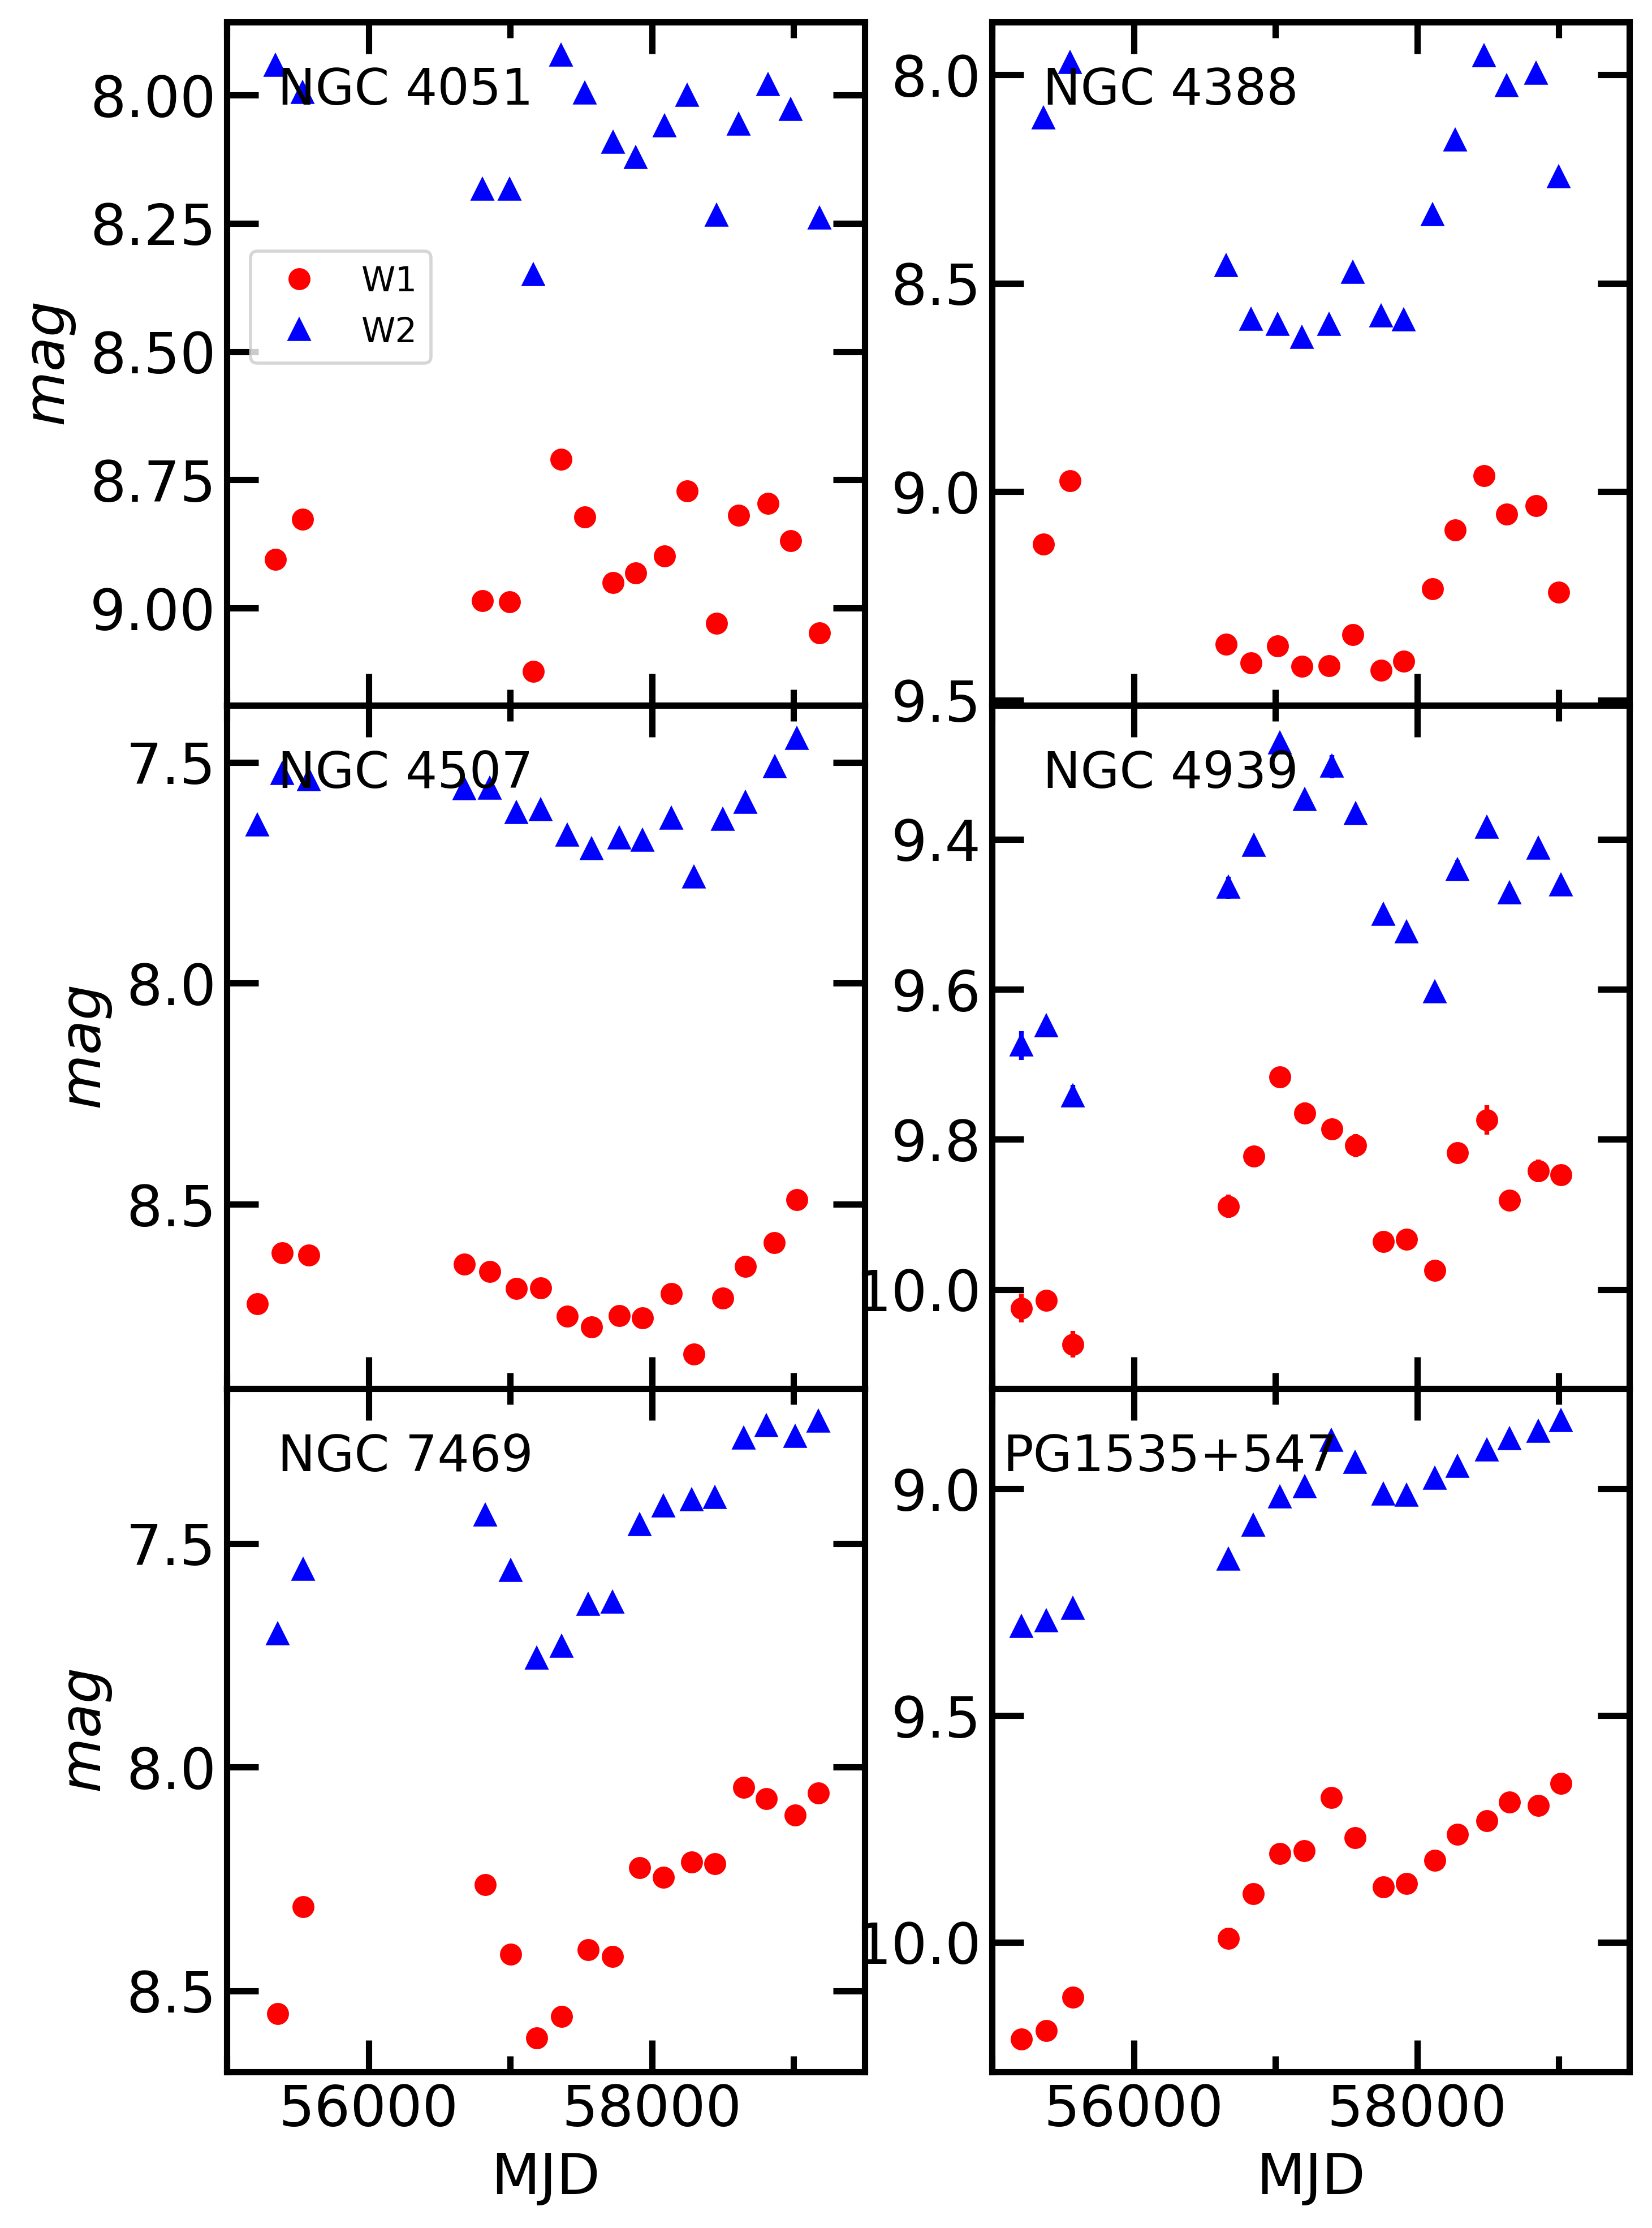
\includegraphics[width=0.6\textwidth]{pic/wisename_varX.png}
    \caption{{\it WISE} light curves of X-ray selected highly variable CLAGNs with $\Delta\,W1$ more than $0.3$ mag. }
    \label{fig:X-CLAGN-lc}
\end{figure}


\subsection{MIR luminosity and color distribution}
The $W1$ magnitude (\texttt{w1mpro} and \texttt{w1mpro\_ep}) and $W2$ magnitude (\texttt{w2mpro} and \texttt{w2mpro\_ep}) are converted from Vega to AB magnitude with $m_{\rm AB} = m_{\rm Vega} + \Delta m$, where $\Delta m$ is 2.699 and 3.339 in $W1$ and $W2$ bands, respectively. Then the MIR luminosity is estimated from the AB magnitude and their luminosity distance. We plot the distribution of variability color ($W1$-$W2$), and the Eddington-scaled $W$1 luminosity ($L_\mathrm{W1}/L_\mathrm{Edd}$) in \autoref{fig:color_ledd}, and \autoref{fig:distribution_ledd}, respectively.

\begin{figure}
\centering
	% To include a figure from a file named example.*
	% Allowable file formats are eps or ps if compiling using latex
	% or pdf, png, jpg if compiling using pdflatex
	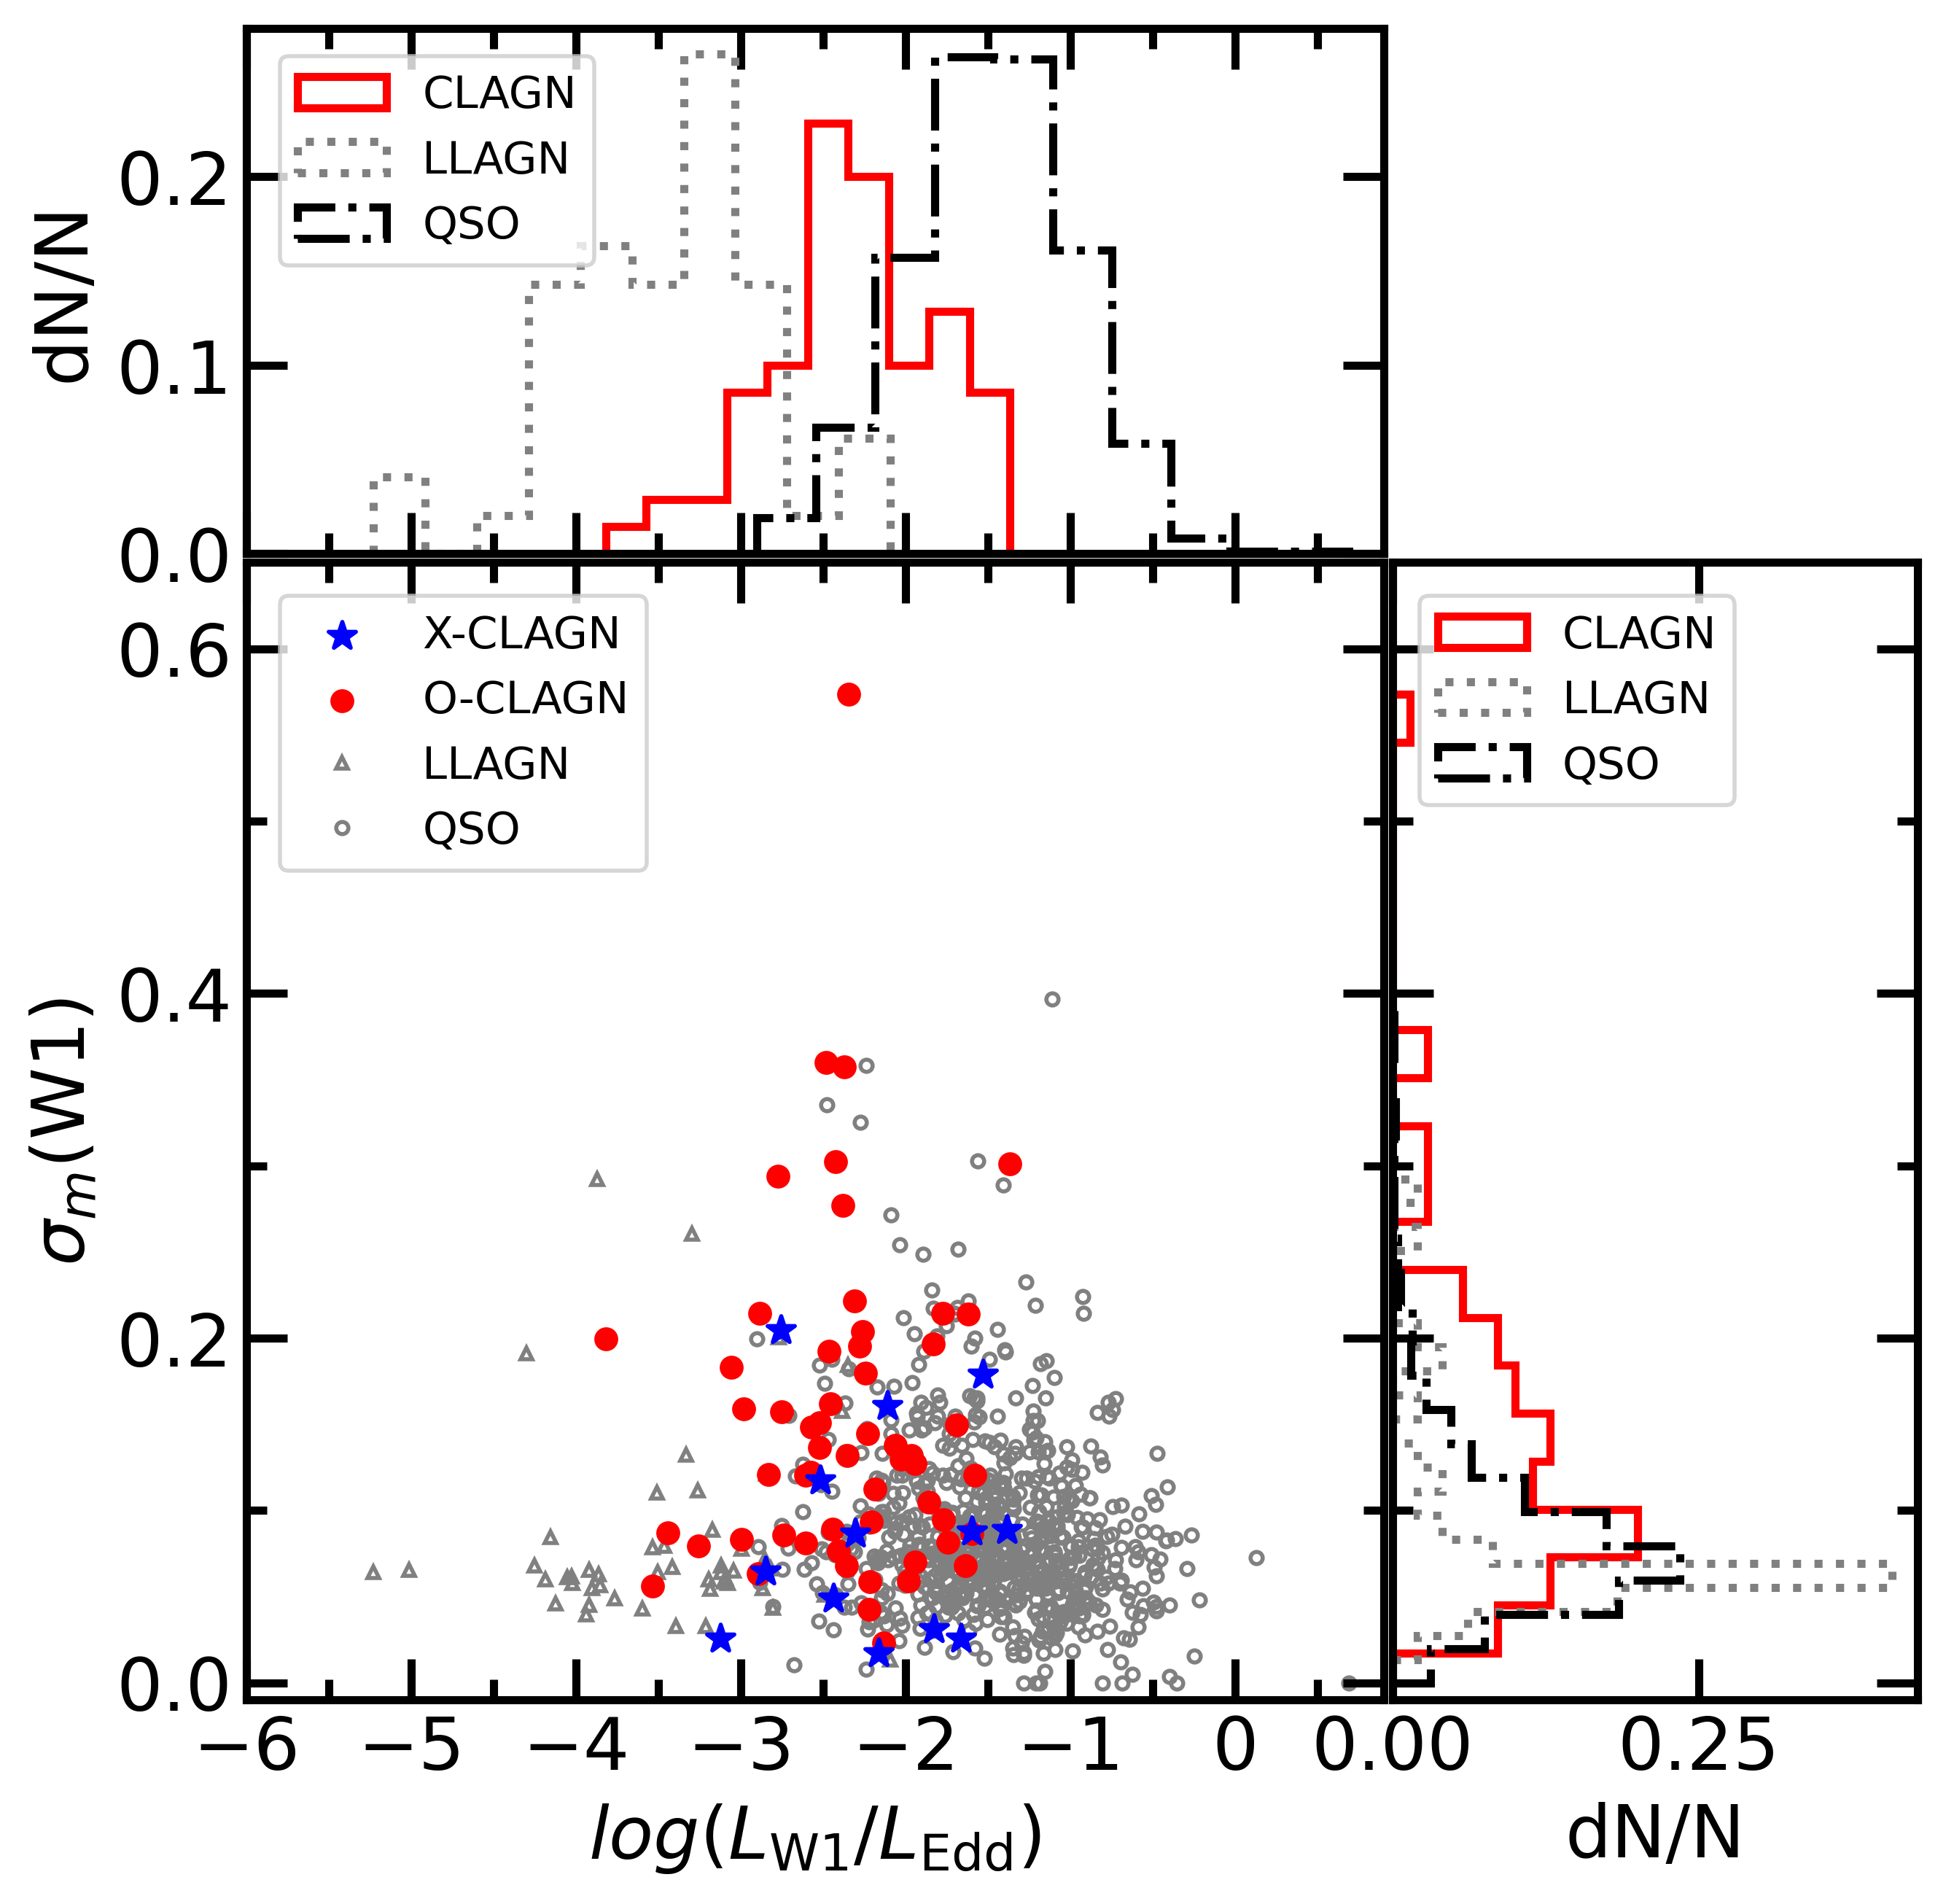
\includegraphics[width=0.45\textwidth]{WISE_var_LW1_Ledd_hist.png}
    \caption{Correlation and distribution of the variability of W1 band and the mean  Eddington-scaled W1 band luminosity for LLAGNs \citep{2009MNRAS.399..349G}, CLAGNs and QSOs \citep{2007ApJ...667..131G}. }
    \label{fig:var_ledd_hist}
\end{figure}

\begin{figure}
\centering
	% To include a figure from a file named example.*
	% Allowable file formats are eps or ps if compiling using latex
	% or pdf, png, jpg if compiling using pdflatex
	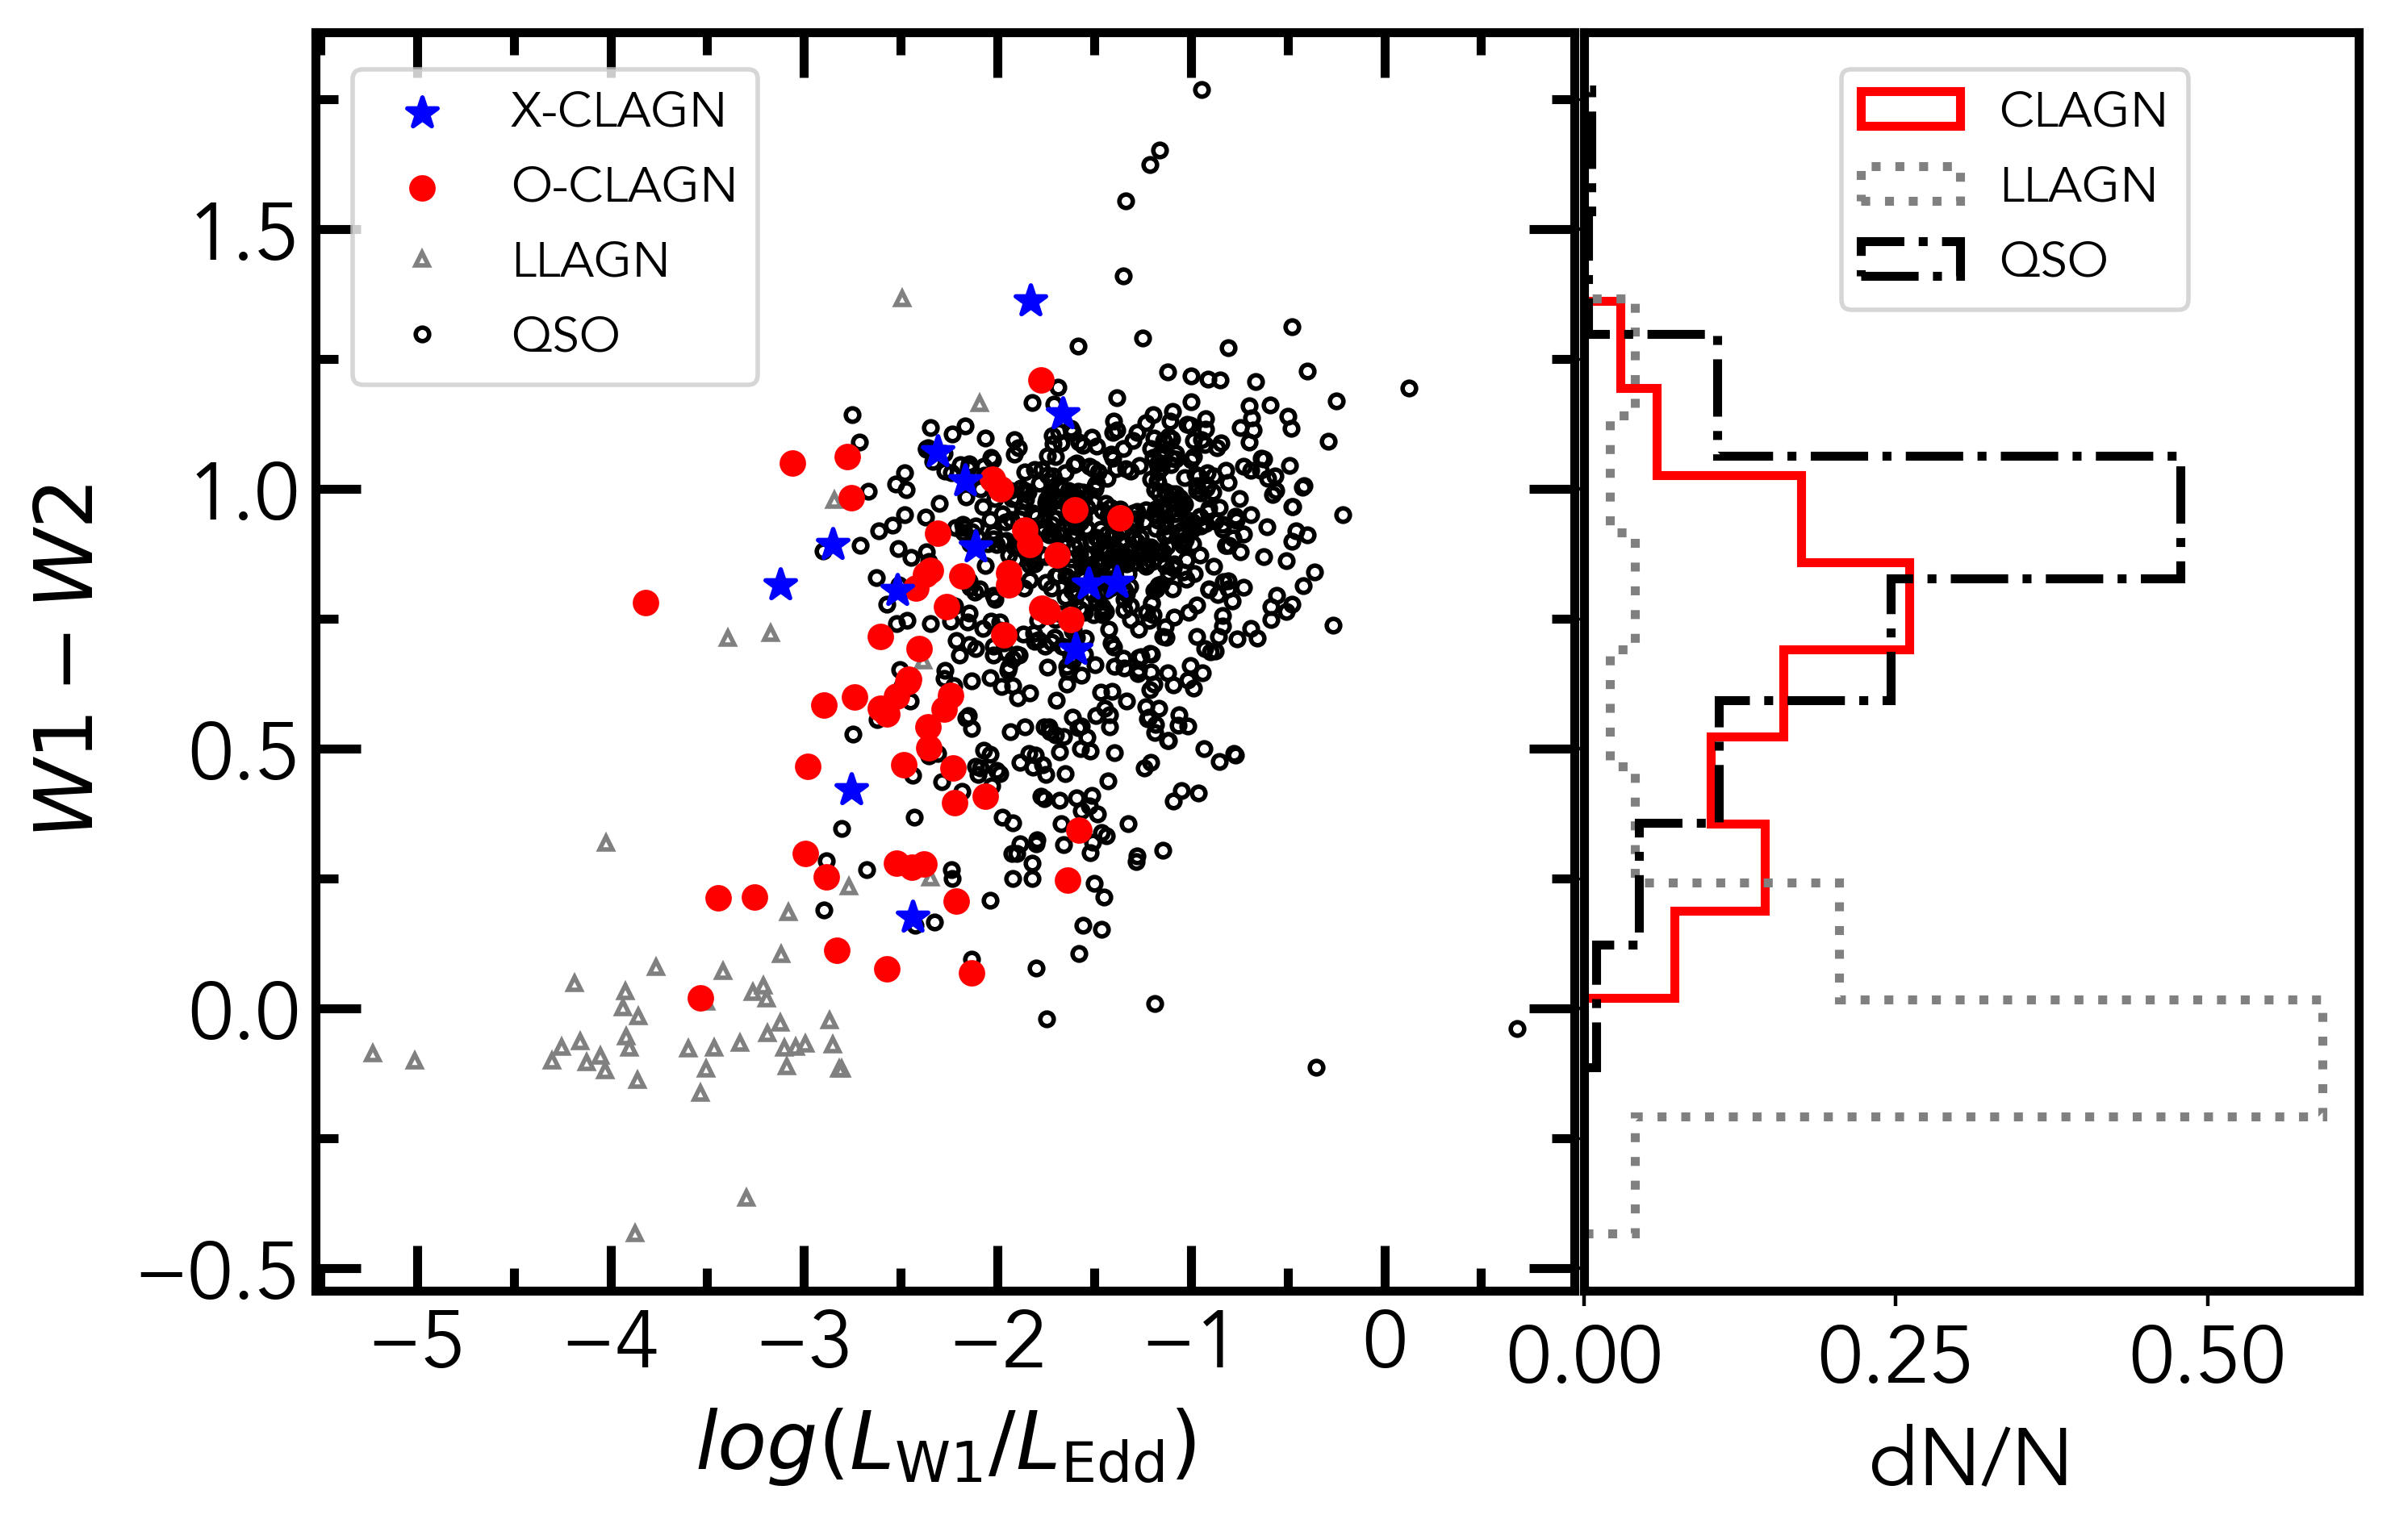
\includegraphics[width=0.45\textwidth]{pic/WISE_W1-W2_LW1_Ledd_hist.png}
    \caption{Correlation of mean $W1-W2$ color and the mean Eddington-scaled W1 band luminosity for LLAGNs\citep{2009MNRAS.399..349G}, CLAGNs and QSOs \citep{2007ApJ...667..131G}. }
    \label{fig:color_ledd}
\end{figure}

\begin{figure}
\centering
	% To include a figure from a file named example.*
	% Allowable file formats are eps or ps if compiling using latex
	% or pdf, png, jpg if compiling using pdflatex
	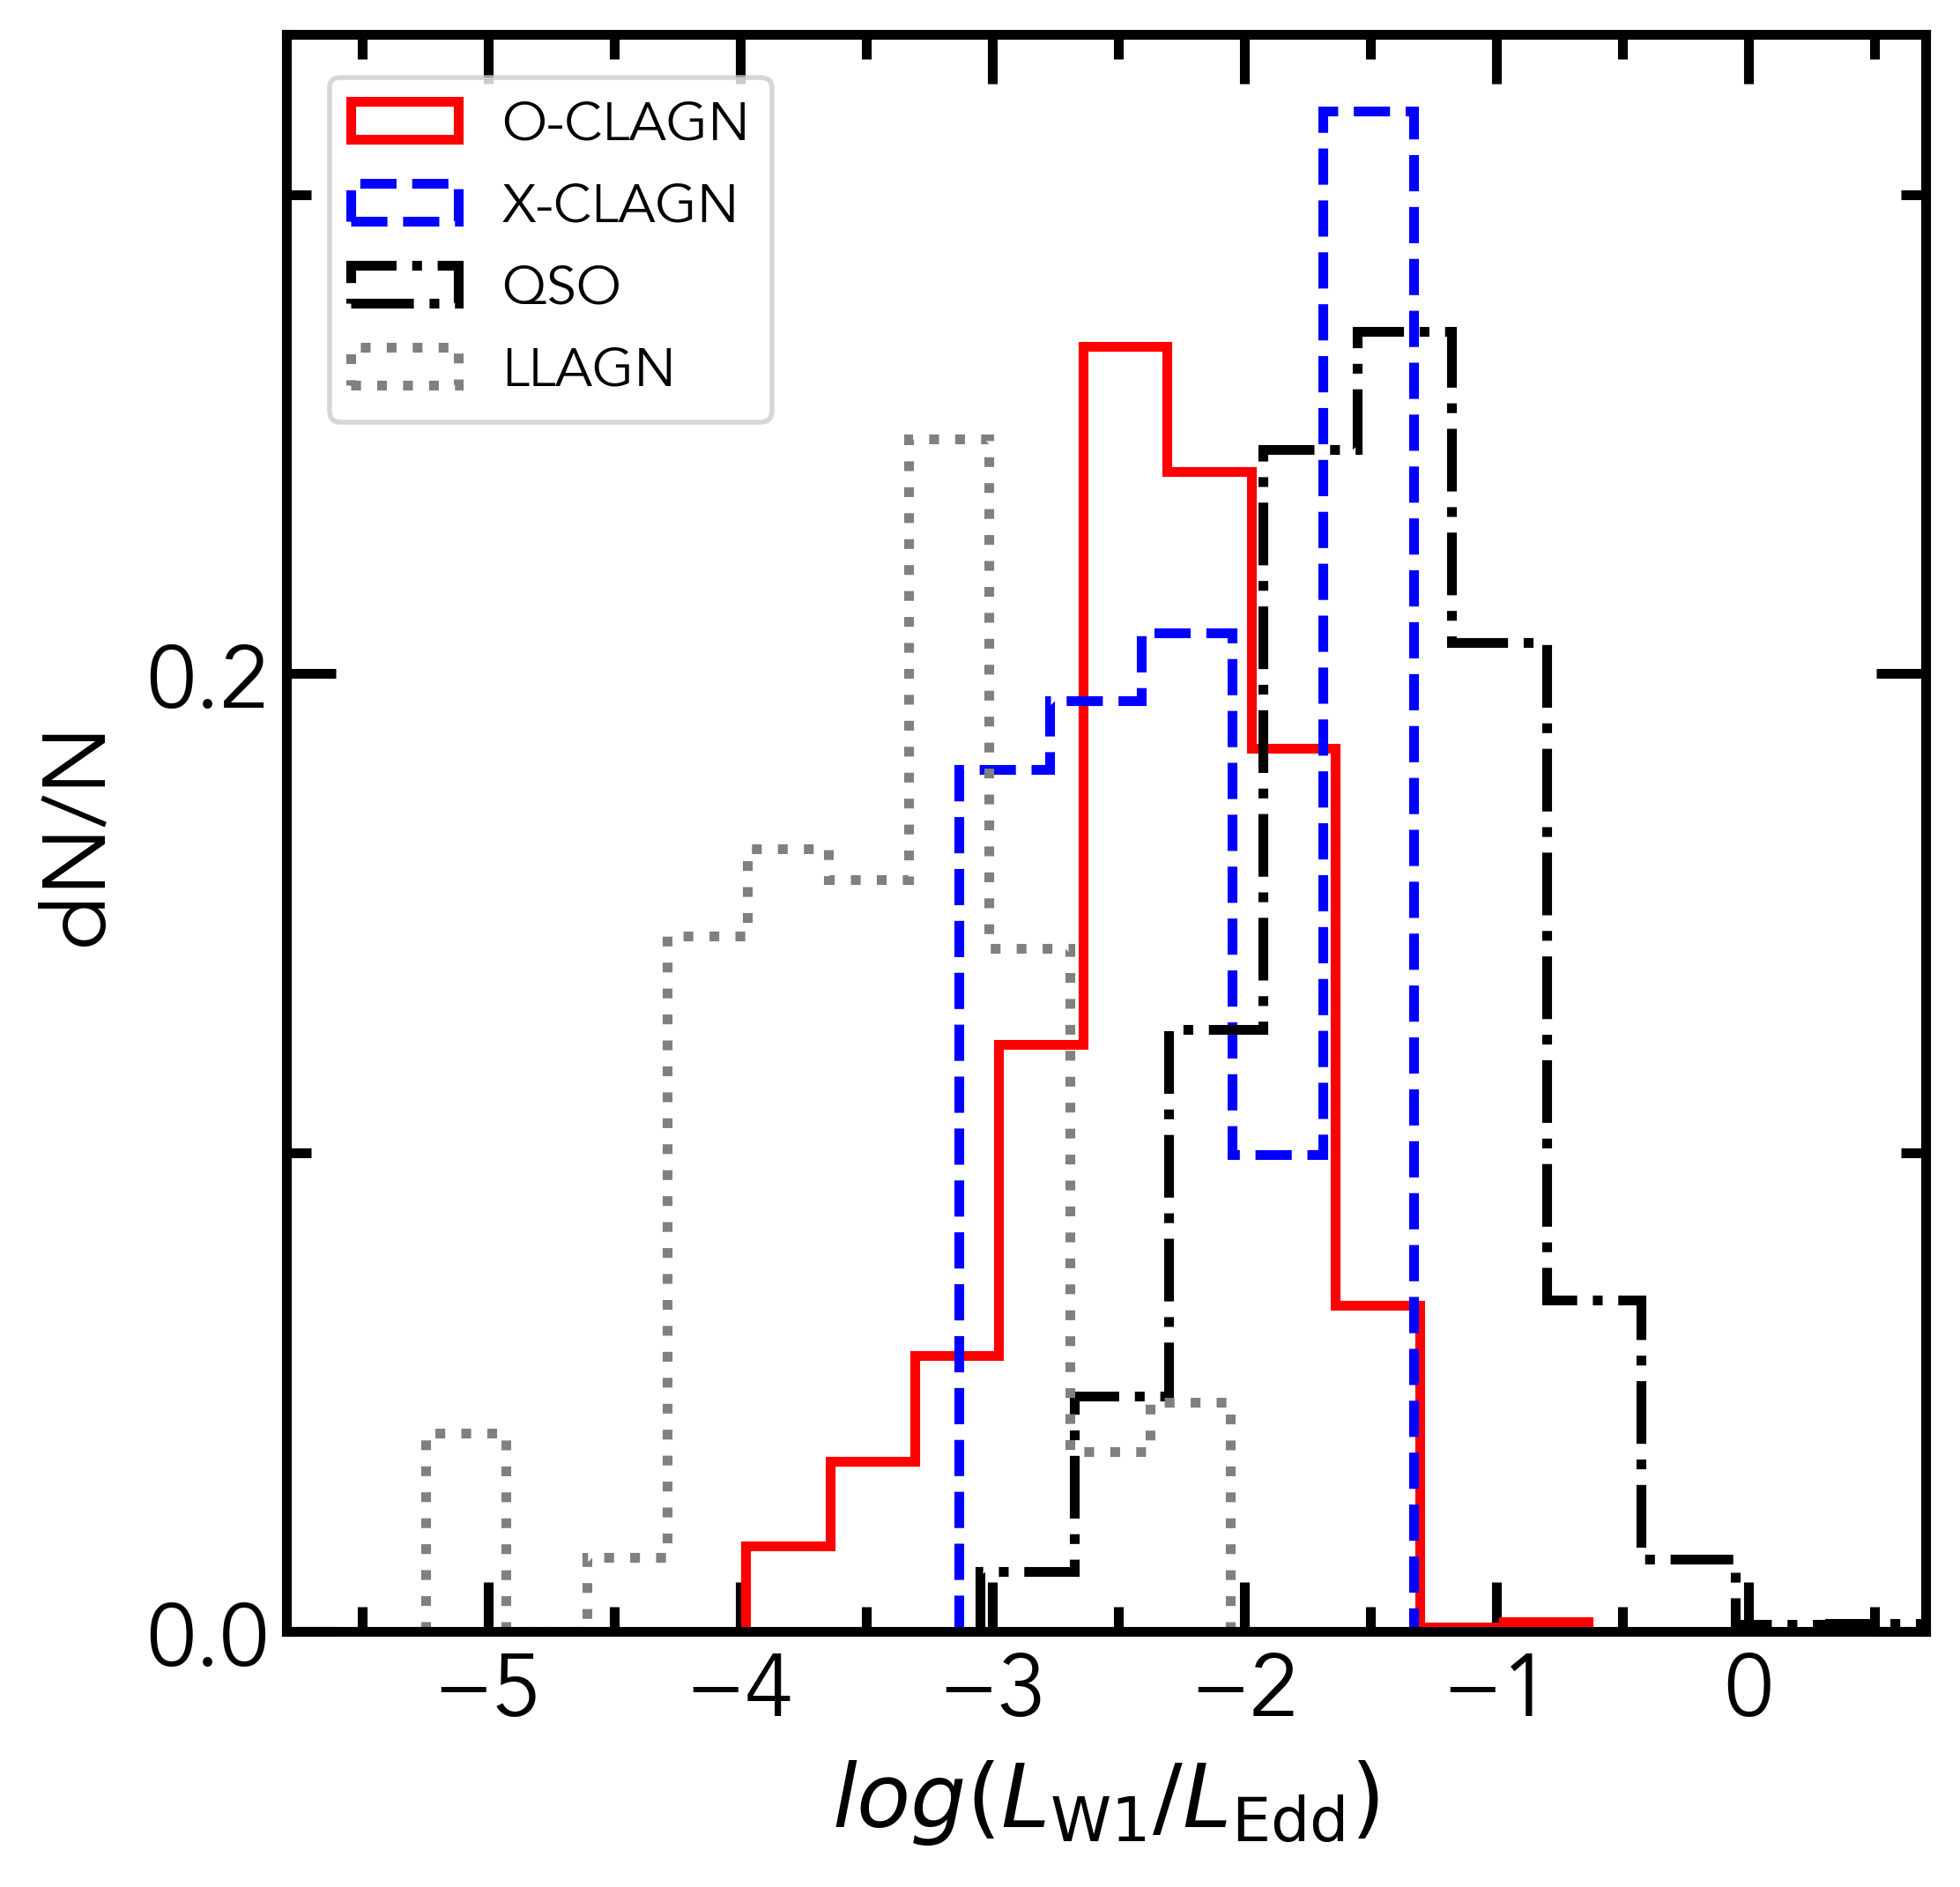
\includegraphics[width=0.45\textwidth]{pic/WISE_LW1_Ledd_hist_rebin_OX.png}
    \caption{Distribution of the Eddington-scaled W1 band luminosity re-binned in each visit for LLAGNs\citep{2009MNRAS.399..349G}, CLAGNs and QSOs \citep{2007ApJ...667..131G}. }
    \label{fig:distribution_ledd}
\end{figure}





\section{dust-reverberation time lag and luminosity relation}
\subsection{time lag analysis}
We used the V band data from the ASAS-SN \citep[All-sky Automated Survey for Supernovae,][]{2014ApJ...788...48S,2017PASP..129j4502K,2019MNRAS.485..961J} and \uvot\, and MIR data from {\it WISE} $W1$ band to estimate the dust echo time lag of several CLAGNs with long-term observational monitoring. We used the interpolation cross correlation function \citep[ICCF;][]{1998PASP..110..660P,2018ascl.soft05032S} in a range of 0--400 days for the first attempt to estimate the dust echo time lag ($\tau$) and then further limited the range according to the posterior of $\tau$. The interpolation time step of 5 days were both applied to optical/X-ray band and $W1$ band light curves. The flux randomization and random subset selection methods were employed with 50000 realizations in the Monte Carlo simulation to estimate the centroid time lag and the uncertainties\footnote{The code \texttt{pyCCF} is available in \url{http://ascl.net/code/v/1868}}. Besides, we used {\sc javelin} algorithm which fits the light curves using a damped random walk (DRW) model with amplitude and time scale of the variability. A top-hat transfer function (TF) is convolved with the driving light curve and the best-fit model parameters such as time lag $\tau$ are found through the Markov Chain Monte Carlo method. We restricted the lag we searched in a range in 0-400 days and width range in 0-400 days in the first attempt. 

\subsubsection{NGC 1566}
We used the combined photometric V band data of NGC 1566 from ASAS-SN  and \uvot\,, and the re-binned $W1$ data in each visit to estimate the dust echo time lag of NGC 1566 due to its high cadence-monitoring observations. We used the tool \textit{uvotsource} to do the aperture photometry for V-band data of \uvot\,. The source aperture radius is 5$\arcsec$ and the background is chosen in a blank region with a much larger radius. ASAS-SN \citep[][]{2018ATel11893....1D} reported the brightening of NGC 1566 around September 2017, which is brightest in July 2018. We found that the flux of NGC 1566 in ASAS-SN are systematically higher than that of \uvot\,, which might be contamination due to the local crowding that changes the light curve by an additive constant in flux   \citep[see ][]{2017PASP..129j4502K}. We determined the average offset between the simultaneous (within 1 day of interval) ASAS-SN and \uvot\, V-band data. Then the ASAS-SN\,V-band 
flux was reduced to the V-band of \uvot\, system by subtracting the offset. We restricted the lag we searched within a range of $0-100$ days for NGC 1566 after the first attempt. We found a significant $\tau$ peak at $\sim 37$ days. We then used {\sc javelin} method to further examine the time lag that we estimated through the ICCF method. We searched for a lag within a same range ($0-100$ days) with the ICCF method. The posterior distribution of lag peaked at $\sim 26$ days. The lag results are roughly consistent within errors for ICCF and {\sc javelin} approach. The result of dust echo time lag analysis for NGC 1566 is shown in \autoref{fig:lag_NGC1566}. We adopted the bolometric luminosity $\sim 8.7\times \, 10^{42} erg\, s^{-1}$ of NGC 1566 using $L_\mathrm{14-195 keV }$ from the 105-Month Swift-BAT All-sky Hard X-Ray Survey reported in \citet{2018ApJS..235....4O} through a bolometric correction of $L_{\mathrm{bol}}=8 \times L_{\mathrm{14-195 keV }}$\citep[e.g.][]{2009MNRAS.392.1124V}. This is consistent with the result ( 0.09--7.11 $\times \, 10^{43} erg\, s^{-1}$) from X-ray luminosity \citep[see][]{2021MNRAS.507..687J} through a bolometric correction of $L_{bol}=20 L_{\mathrm{2-20 keV}}$ \citep[e.g.][]{2009MNRAS.392.1124V}.


\subsubsection{Mrk 6}
Similarly, we used the data from ASAS-SN and the re-binned $W1$ data to estimate dust echo time lag for Mrk 6. The ASAS-SN V band data was binned in 30 days. We restricted the lag we searched within a range of $0-400$ days in ICCF method and found a peak at $\sim$142 days. Then we used {\sc javelin} method to examine the time lag. We find multiple peaks in the posterior of the time lag and two peaks of width (one is 0 day, another one is around 300 days) in the first attempt. We restricted the lag with a range in 0-250 days and width range in 180-400 days. The posterior distribution of lag peaked at $\sim$170 days, which is roughly consistent with the ICCF approach. The result of dust echo time lag analysis for Mrk 6 is shown in \autoref{fig:lag_Mrk6}. We adopted the bolometric luminosity $\sim 3.9\times \, 10^{44} erg\, s^{-1}$ of Mrk 6 using $L_\mathrm{14-195 keV }$ reported in \citet{2018ApJS..235....4O} through a bolometric correction of $L_{\mathrm{bol}}=8 \times L_{\mathrm{14-195 keV }}$.




\subsubsection{Mrk 926}
We used the data from ASAS-SN and the re-binned $W1$ data to estimate dust echo time lag for Mrk 926. The peaks of lag are $\sim$214 and $\sim$242 days for ICCF and {\sc javelin} approach. The result of dust echo time lag analysis for Mrk 926 is shown in \autoref{fig:lag_Mrk926}. We adopted the bolometric luminosity $\sim 4.6\times \, 10^{45} erg\, s^{-1}$ of Mrk 926 using $L_\mathrm{14-195 keV }$ reported in \citet{2018ApJS..235....4O} through a bolometric correction of $L_{\mathrm{bol}}=8 \times L_{\mathrm{14-195 keV }}$.


\subsubsection{NGC 7469}
We used the data from ASAS-SN and the re-binned $W1$ data to estimate dust echo time lag for NGC 7469. We extracted data between MJD 56500 and 58500 in observational overlap. We found the time lag peaked at $\sim$131 days for ICCF approach and $\sim$146 days for {\sc javelin} approach. The result of dust echo time lag analysis for NGC 7469 is shown in \autoref{fig:lag_NGC7469}. We adopted the bolometric luminosity $\sim 3.4\times \, 10^{44} erg\, s^{-1}$ of NGC 7469 using $L_\mathrm{14-195 keV }$ reported in \citet{2018ApJS..235....4O} through a bolometric correction of $L_{\mathrm{bol}}=8 \times L_{\mathrm{14-195 keV }}$. 


\subsubsection{PG 1535+547}
We used the data from ASAS-SN and the re-binned $W1$ data to estimate dust echo time lag for PG 1535+547. We extracted data between MJD 56200 and 58300 in observational overlap. The ASAS-SN V band data was binned in 30 days. We restricted the lag we searched within a range of $0-250$ days for ICCF approach. We found the time lag peaked at $\sim$153 days. We restricted the lag we searched within a range of $50-250$ days and width within a range of $0-100$ days for {\sc javelin} approach. The time lag peaked at$\sim$167 days for {\sc javelin} approach. The result of dust echo time lag analysis for PG 1535+547 is shown in \autoref{fig:lag_PG1535}. Since PG 1535+547 was not included in the 105-Month \bat\, survey, we adopted the bolometric luminosity $\sim 1.4\times \, 10^{45} erg\, s^{-1}$ of PG 1535+547 estimated from [O~{\small III}] line by \citet{2006ApJ...653..137Z}.

\begin{figure}
\centering
	% To include a figure from a file named example.*
	% Allowable file formats are eps or ps if compiling using latex
	% or pdf, png, jpg if compiling using pdflatex
	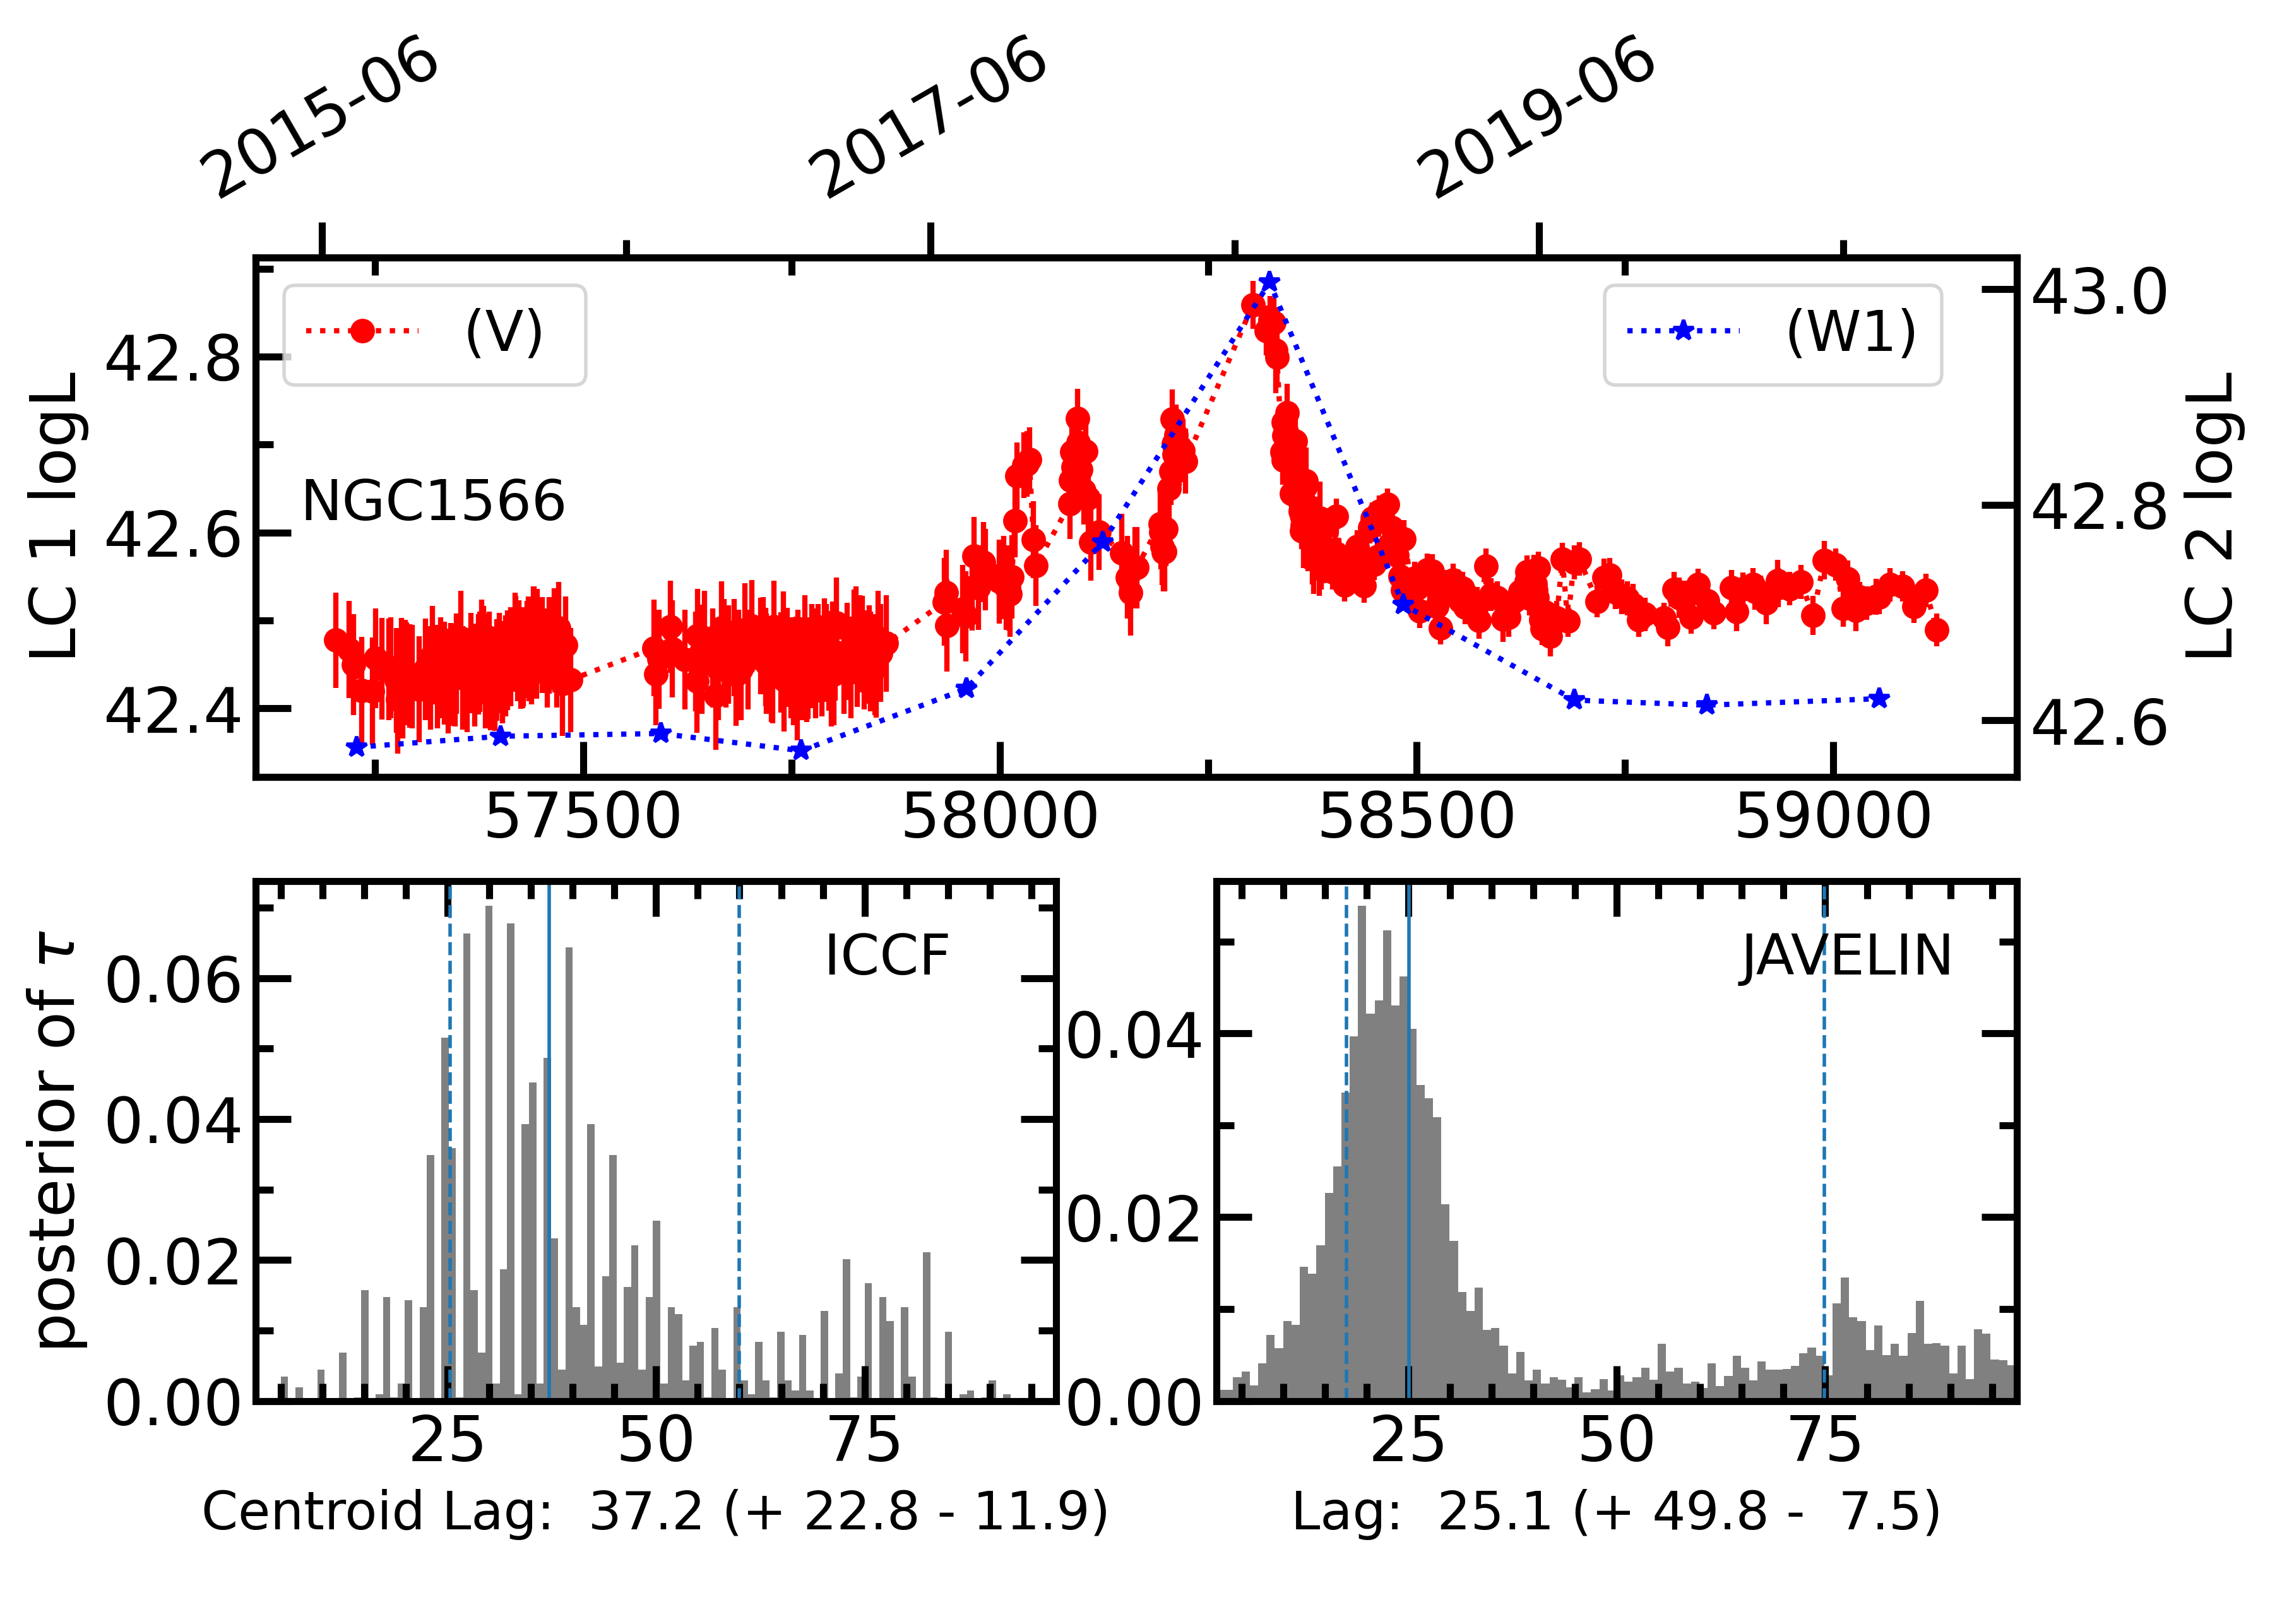
\includegraphics[width=0.5\textwidth]{pic/NGC1566_lag.png}
    \caption{Dust-reverberation time lag analysis for NGC 1566. }
    \label{fig:lag_NGC1566}
\end{figure}
\begin{figure}
\centering
	% To include a figure from a file named example.*
	% Allowable file formats are eps or ps if compiling using latex
	% or pdf, png, jpg if compiling using pdflatex
	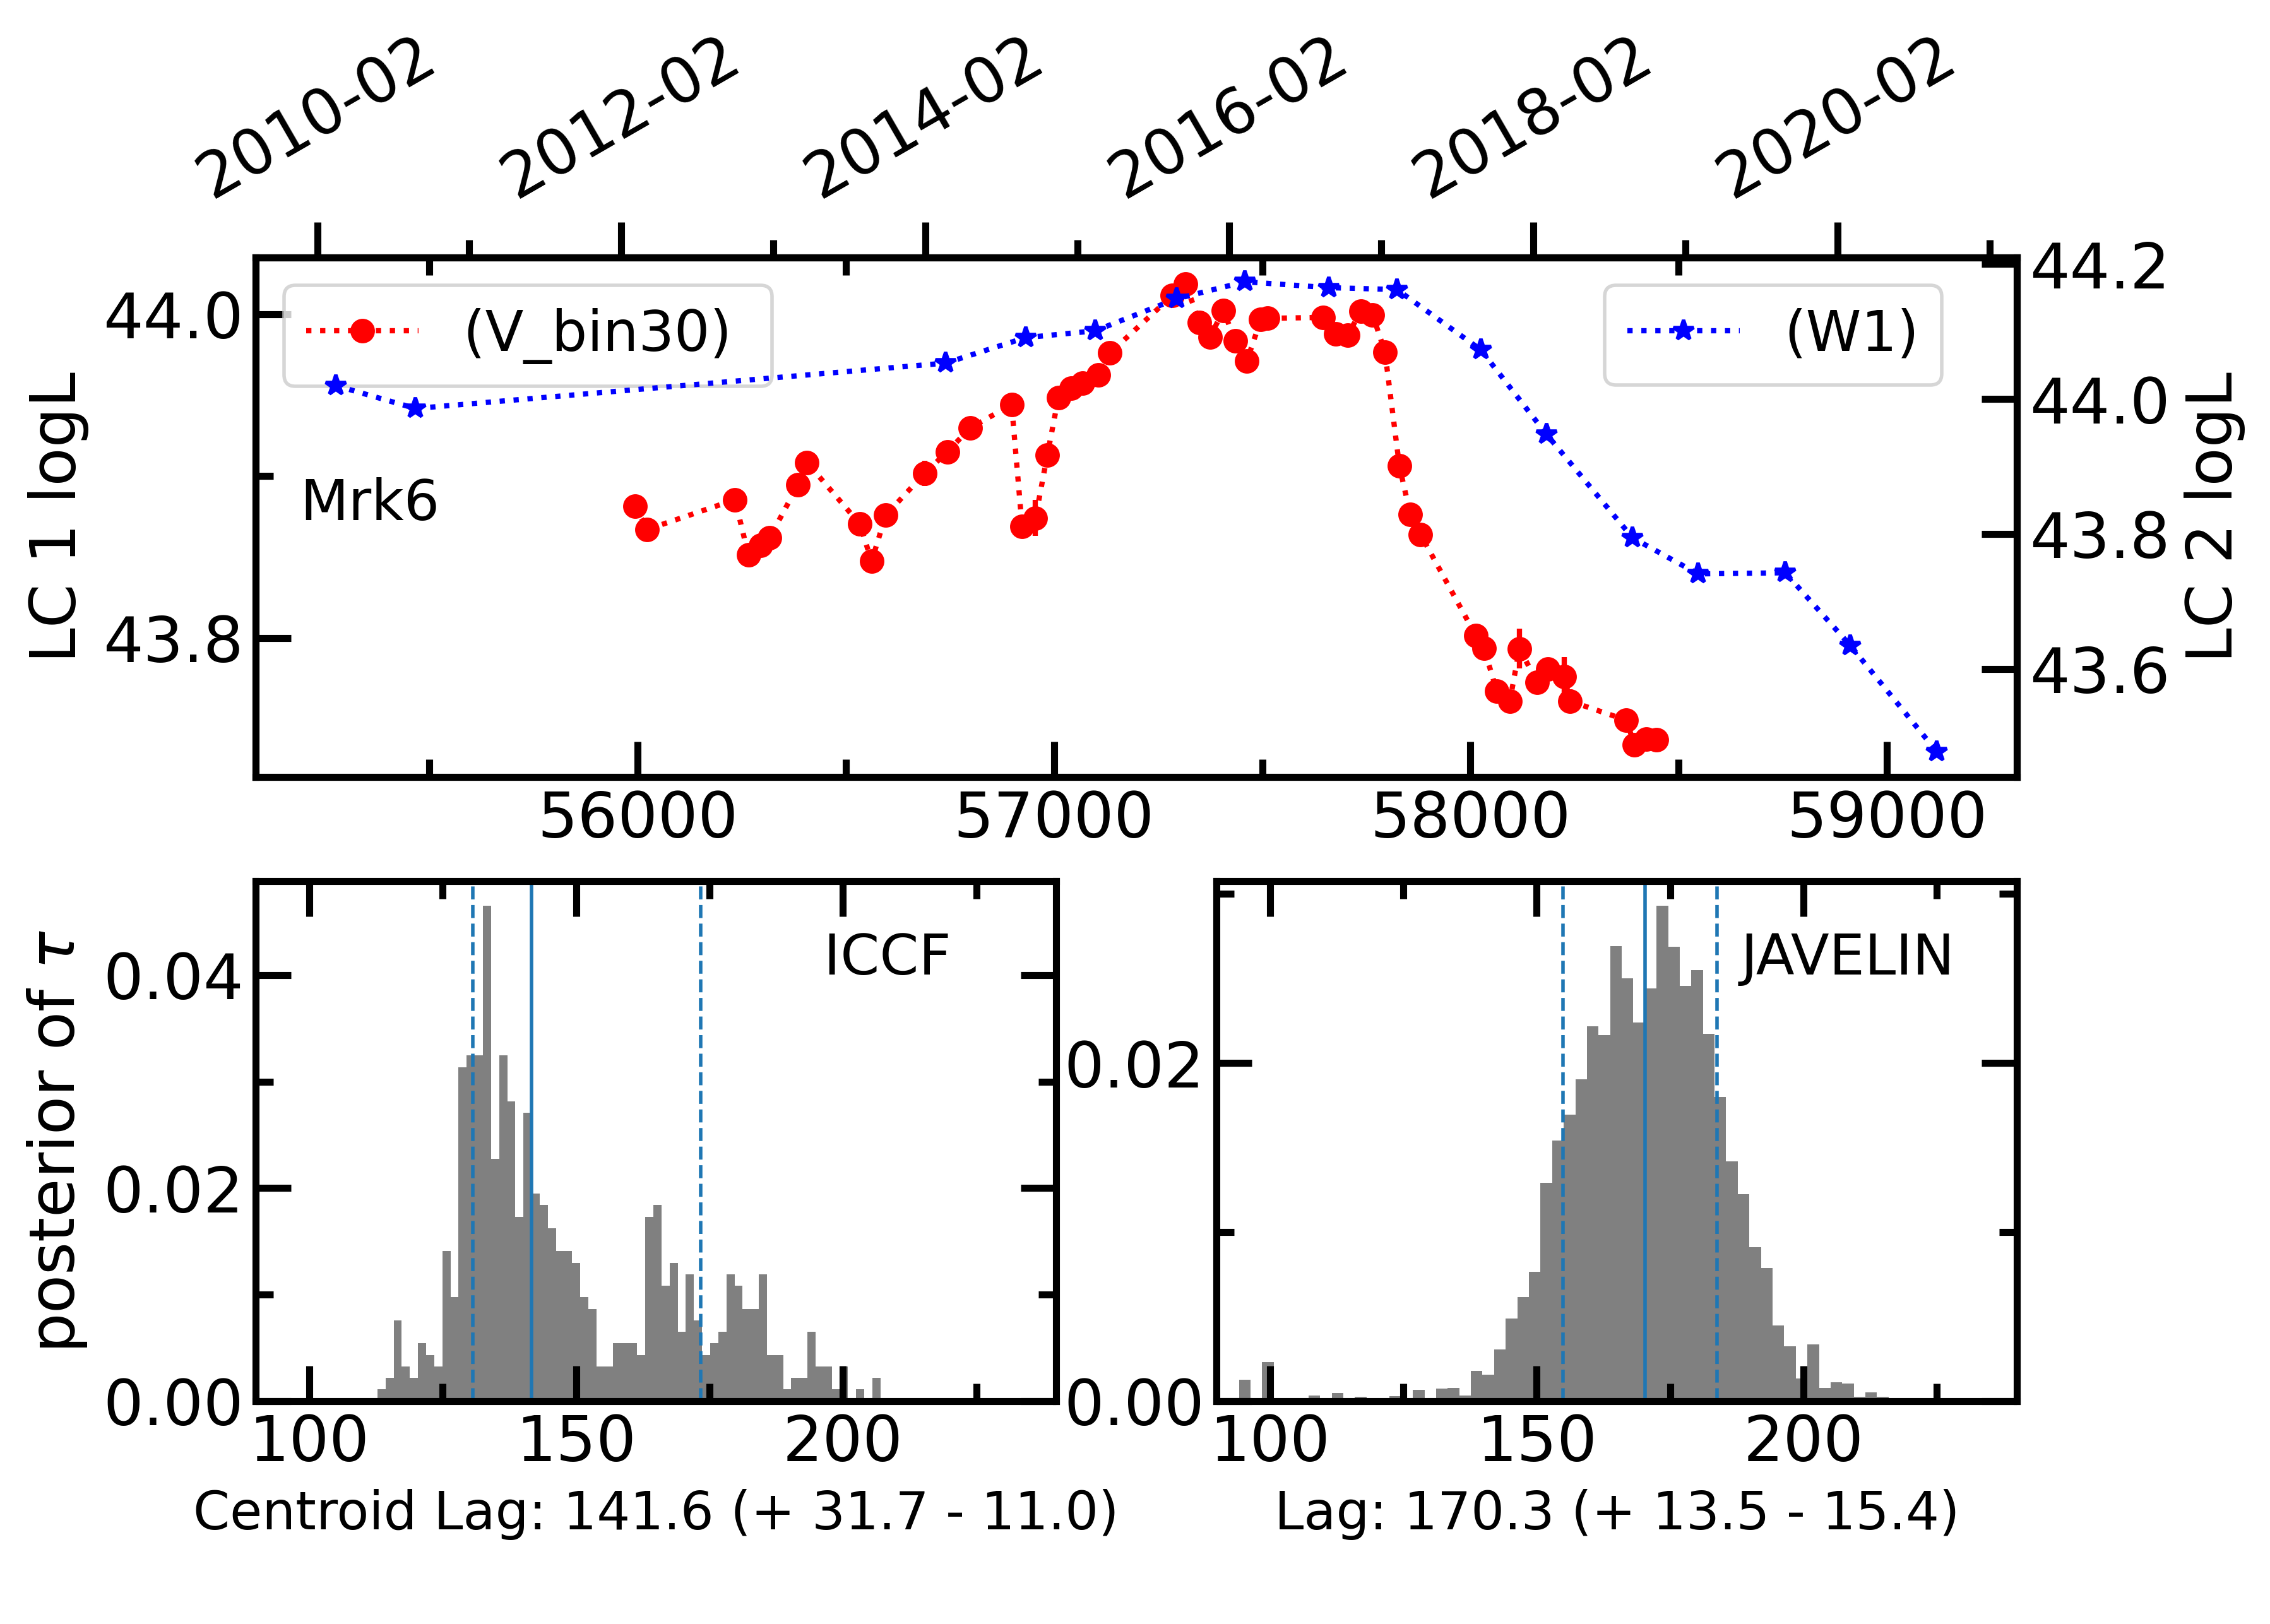
\includegraphics[width=0.5\textwidth]{pic/Mrk6lag1.png}
    \caption{Dust-reverberation time lag analysis for Mrk 6. }
    \label{fig:lag_Mrk6}
\end{figure}
\begin{figure}
\centering
	% To include a figure from a file named example.*
	% Allowable file formats are eps or ps if compiling using latex
	% or pdf, png, jpg if compiling using pdflatex
	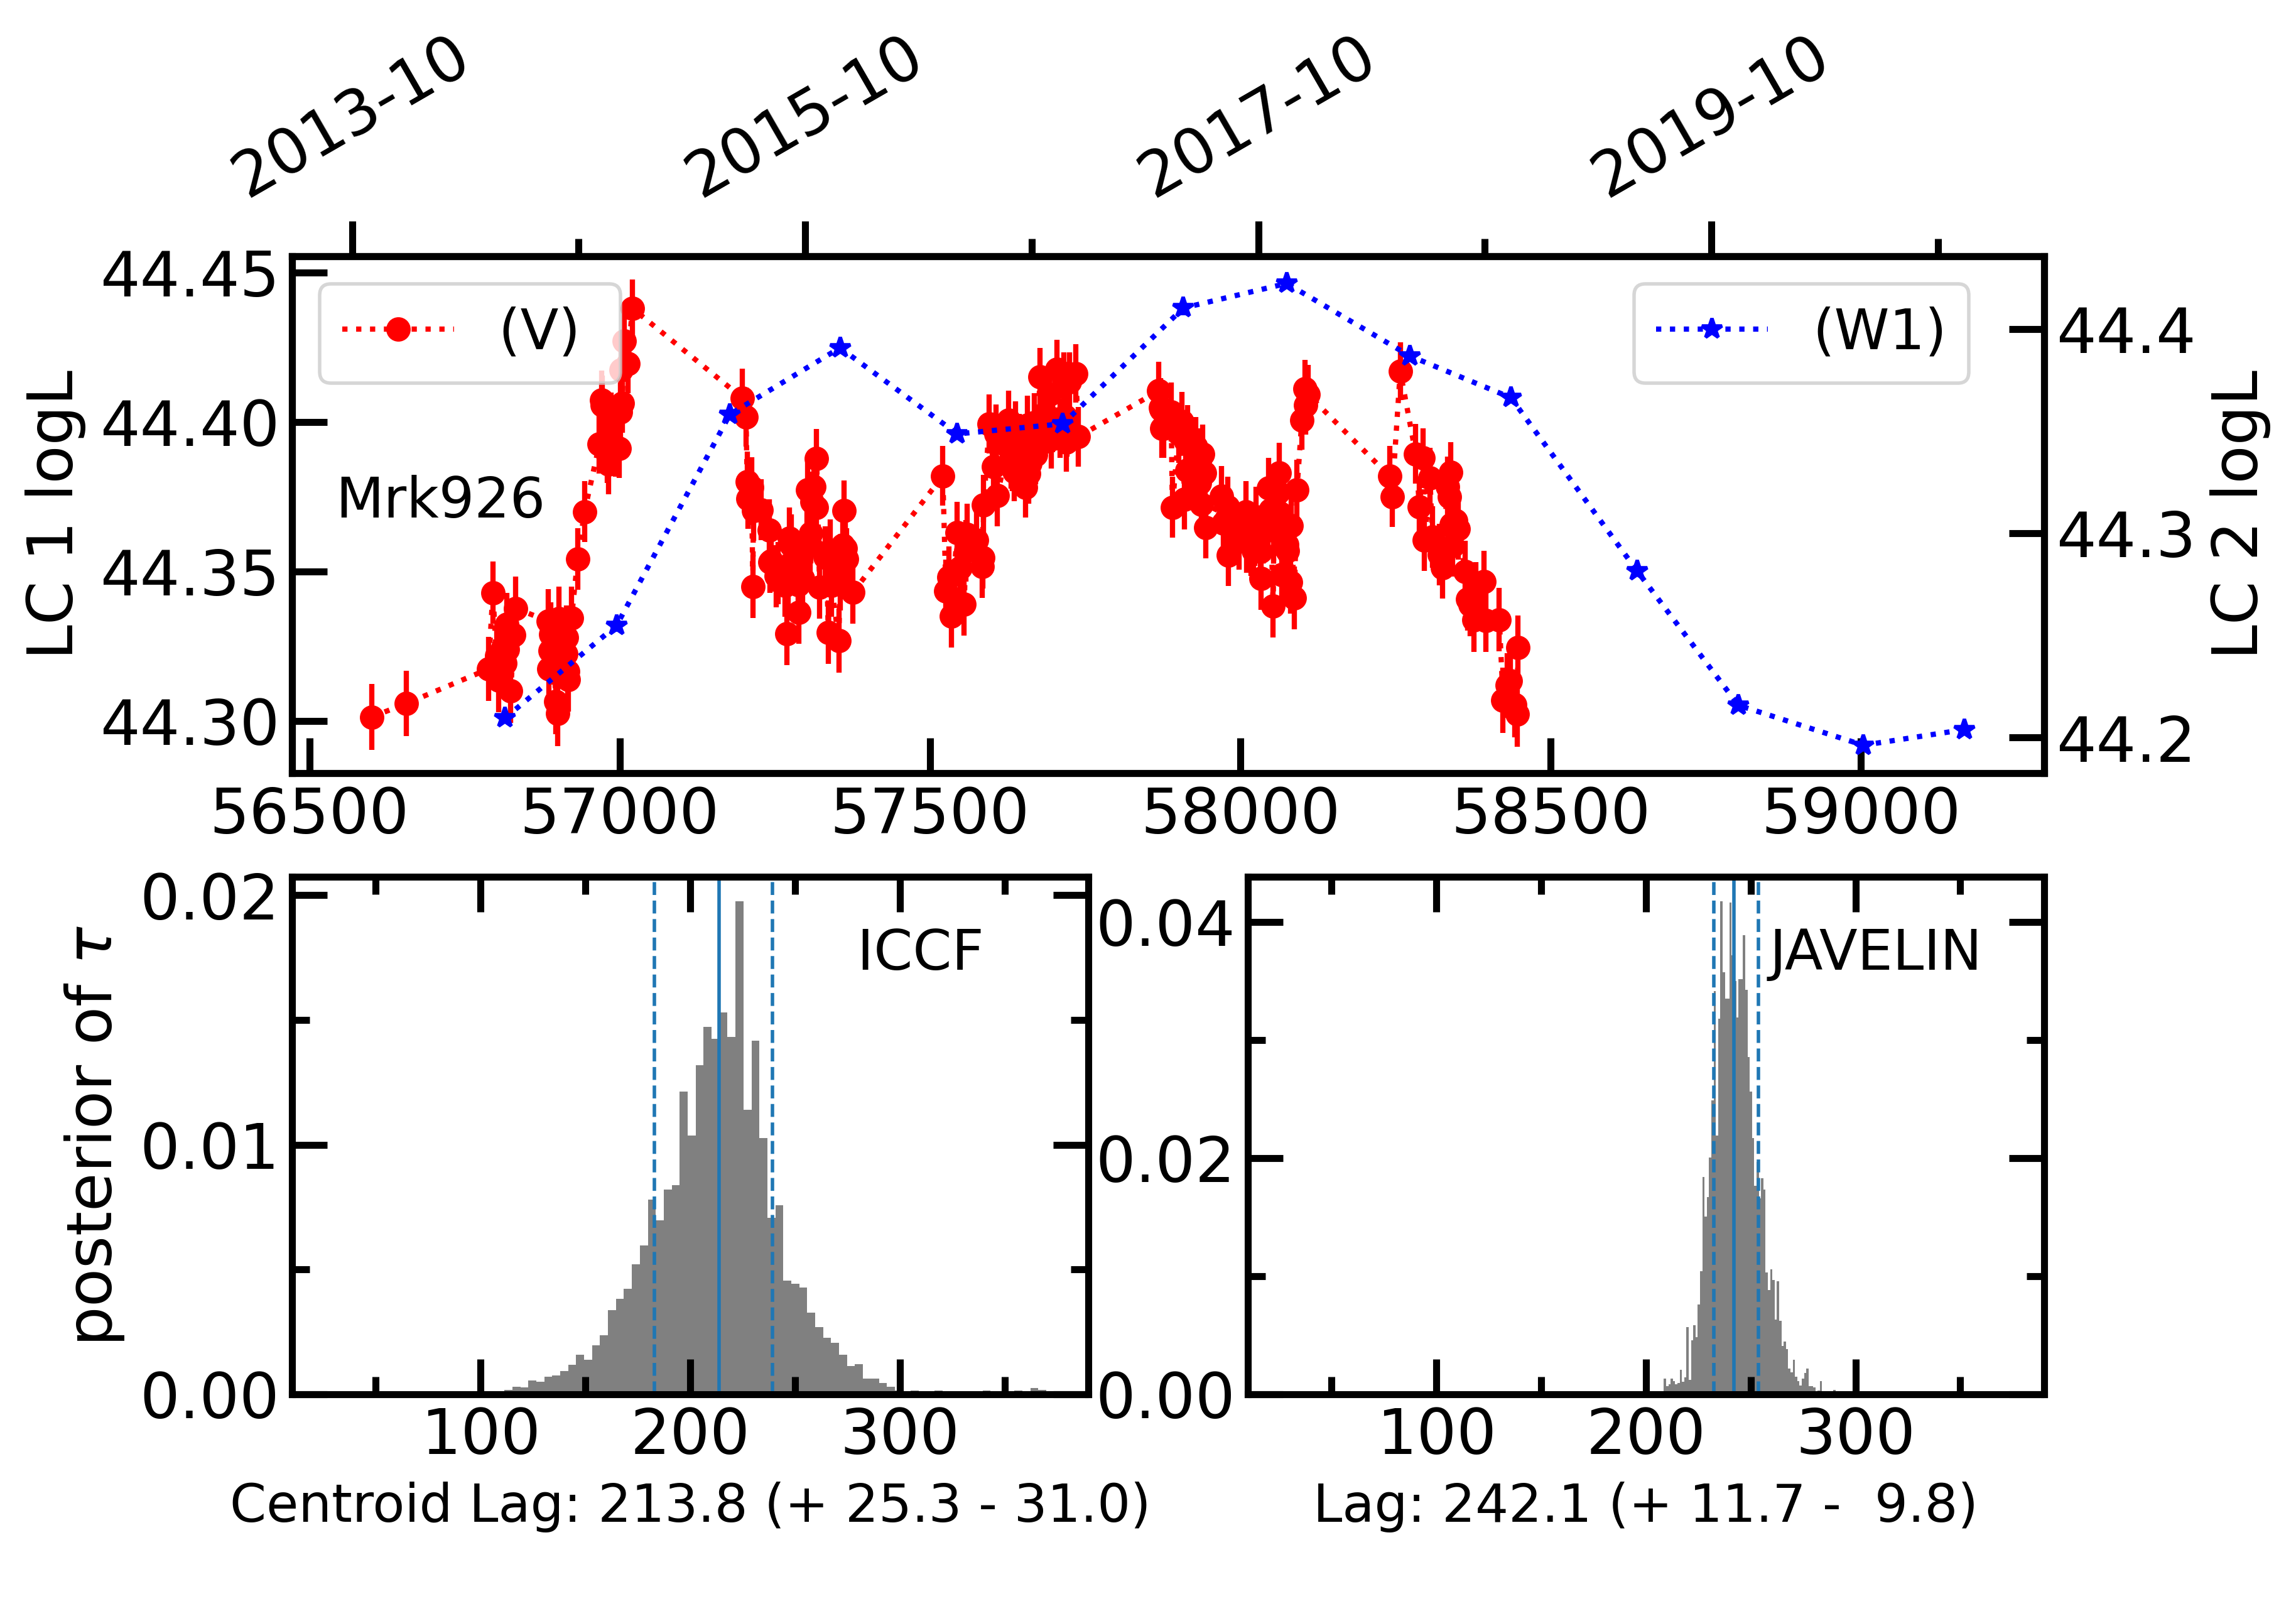
\includegraphics[width=0.5\textwidth]{pic/Mrk926lag.png}
    \caption{Dust-reverberation time lag analysis for Mrk 926. }
    \label{fig:lag_Mrk926}
\end{figure}
\begin{figure}
\centering
	% To include a figure from a file named example.*
	% Allowable file formats are eps or ps if compiling using latex
	% or pdf, png, jpg if compiling using pdflatex
	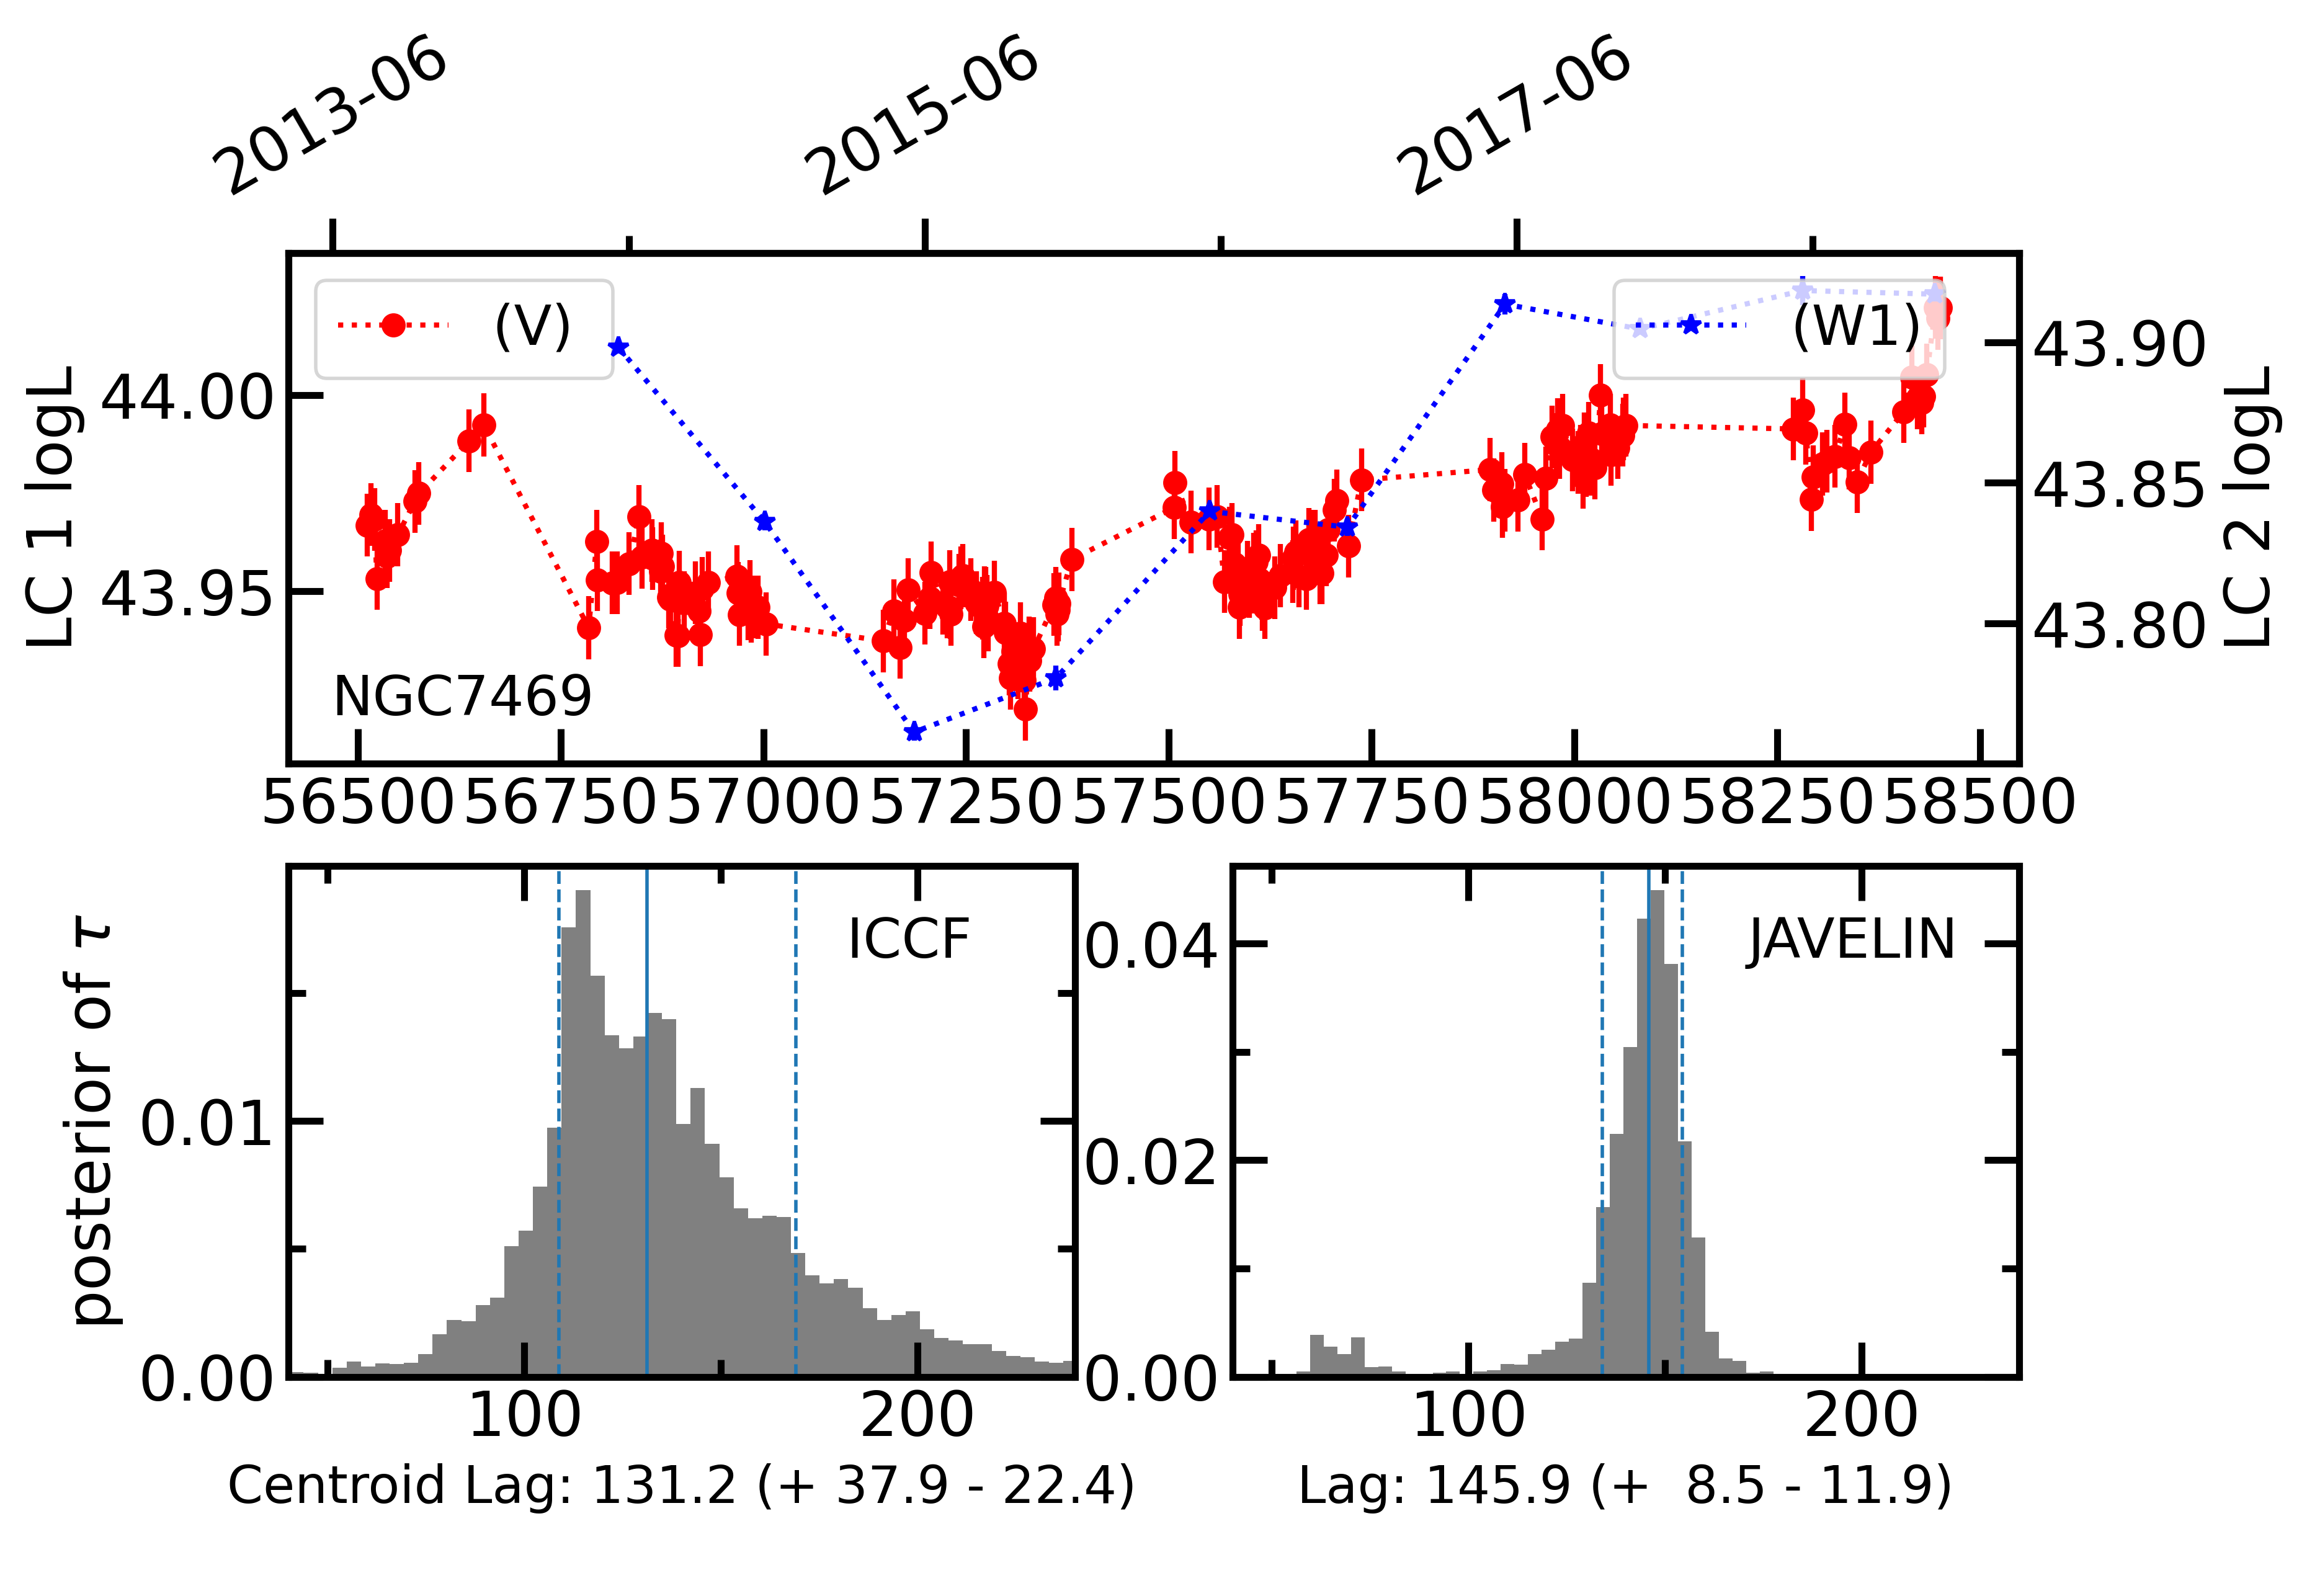
\includegraphics[width=0.5\textwidth]{pic/NGC7469lag.png}
    \caption{Dust-reverberation time lag analysis for NGC 7469. }
    \label{fig:lag_NGC7469}
\end{figure}
\begin{figure}
\centering
	% To include a figure from a file named example.*
	% Allowable file formats are eps or ps if compiling using latex
	% or pdf, png, jpg if compiling using pdflatex
	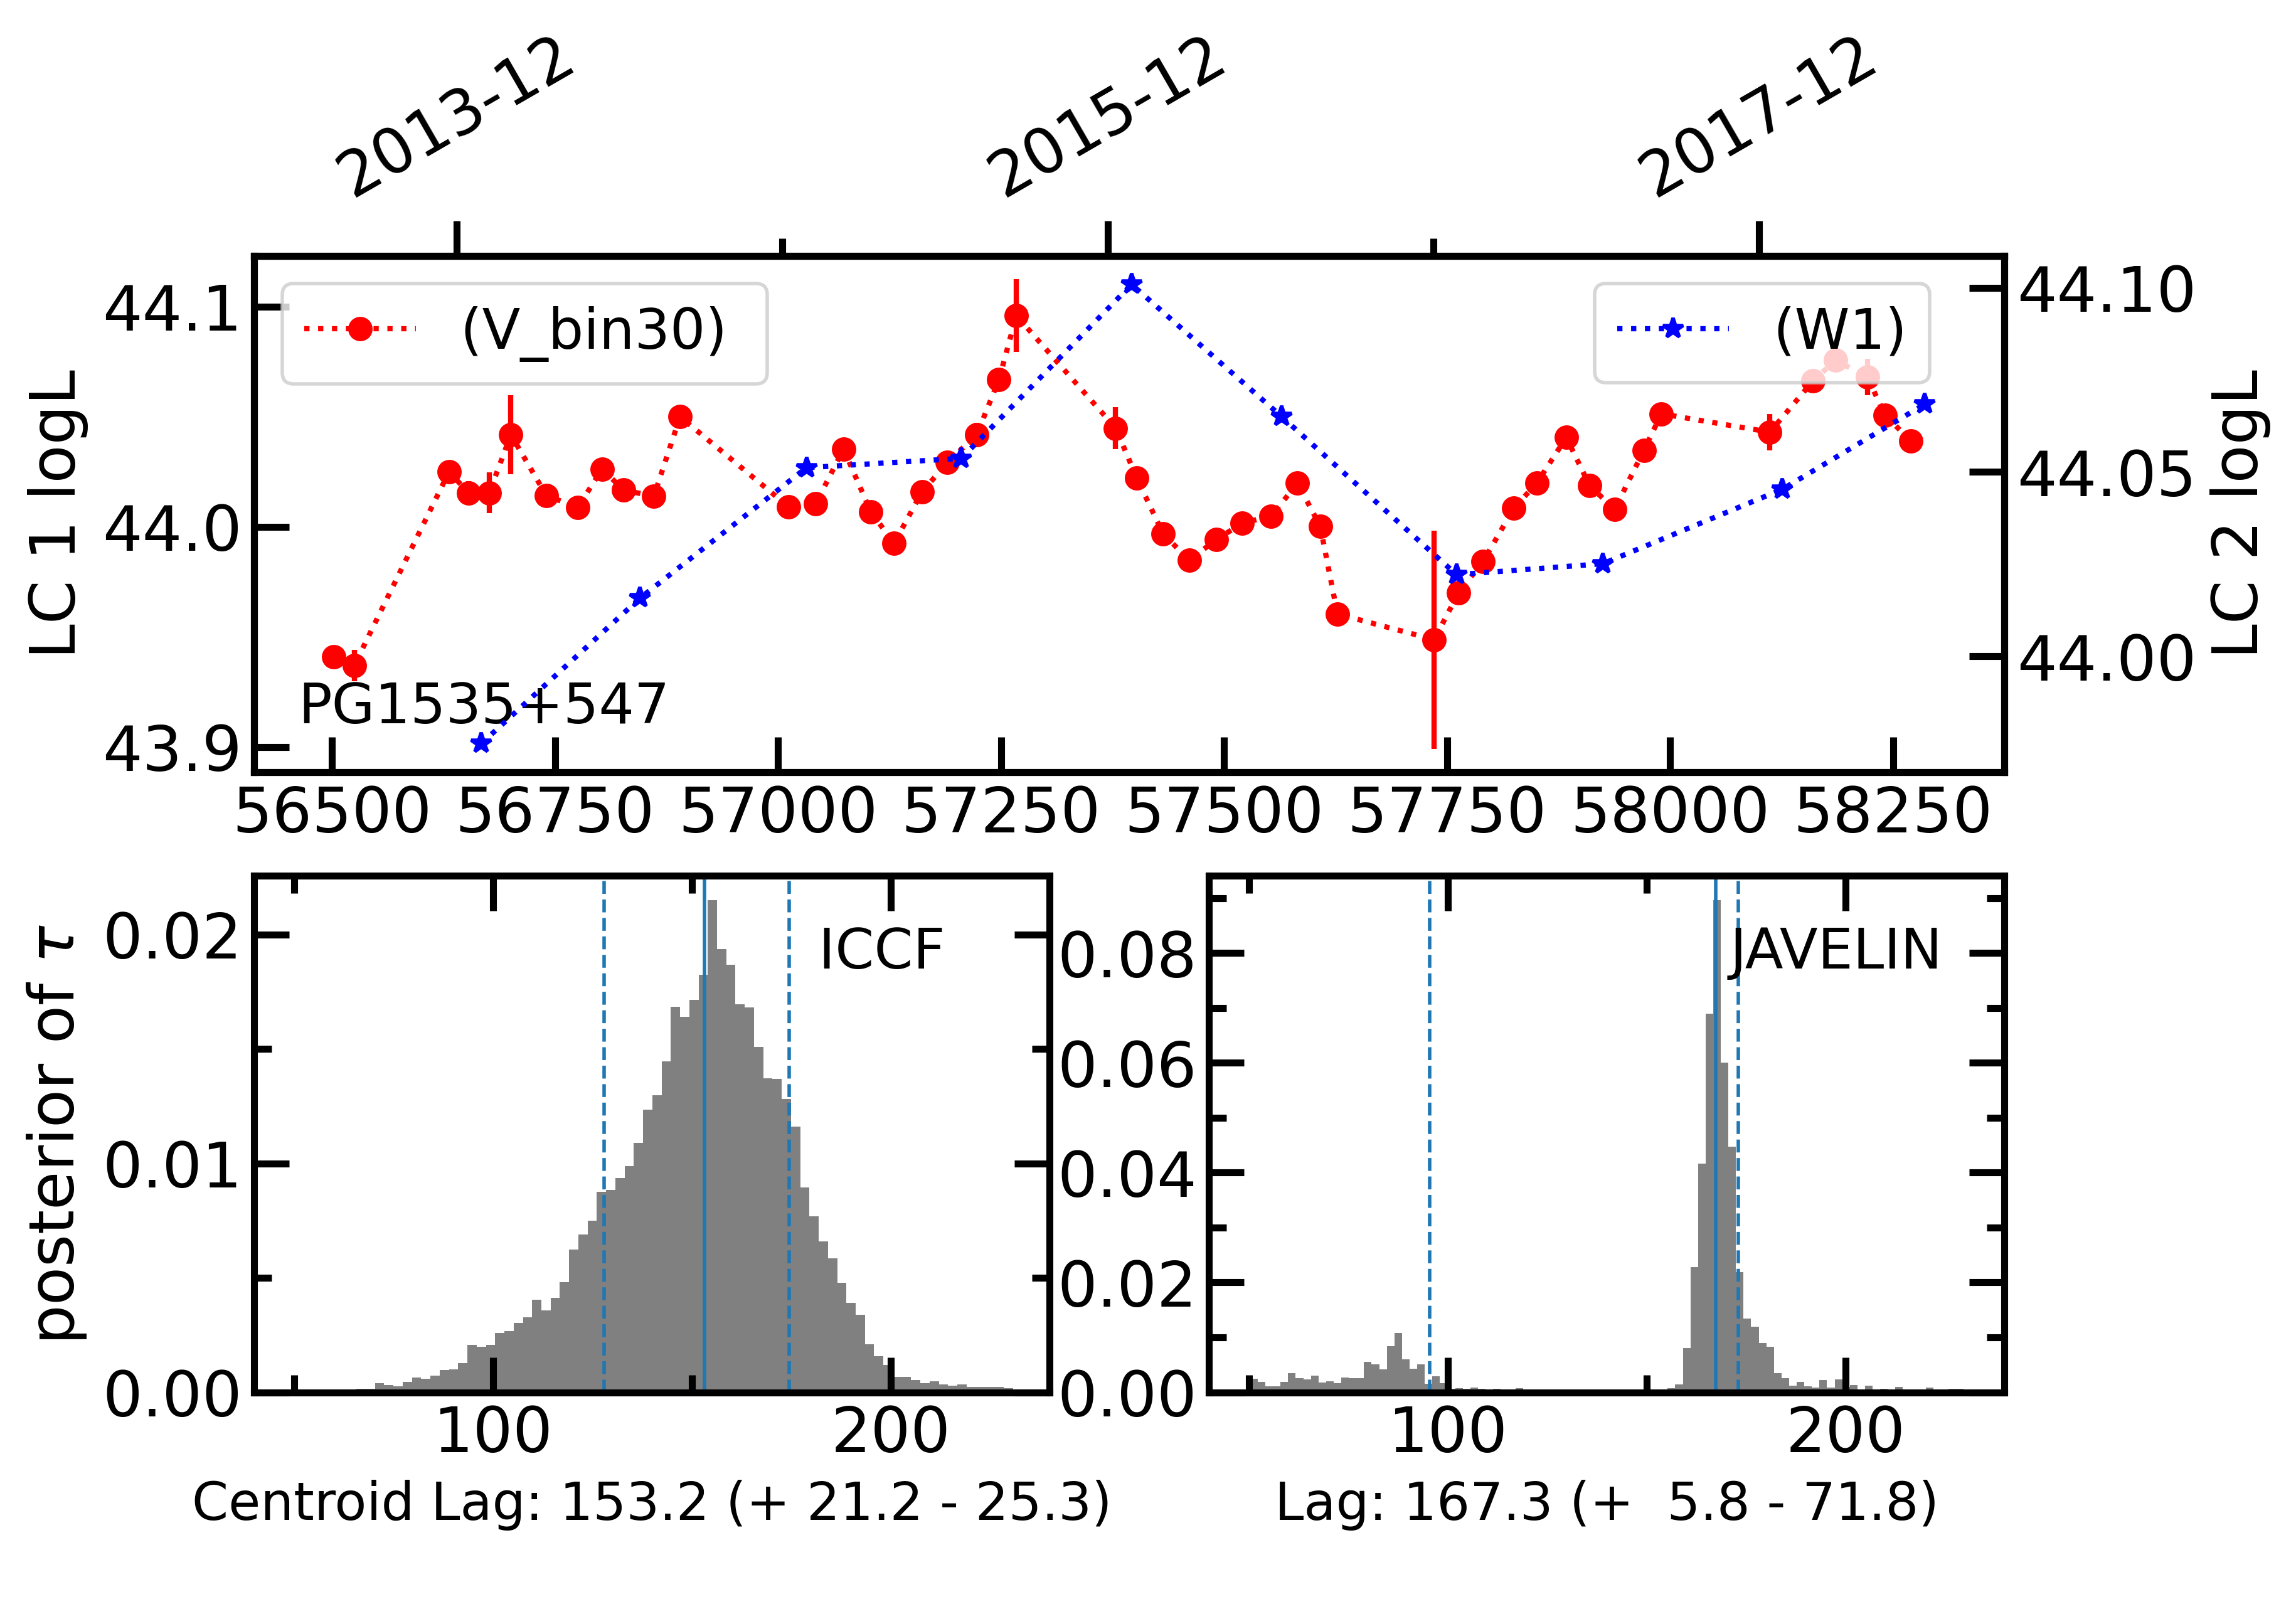
\includegraphics[width=0.5\textwidth]{pic/PG1535p547lag1.png}
    \caption{Dust-reverberation time lag analysis for PG 1535+547. }
    \label{fig:lag_PG1535}
\end{figure}






\subsection{$\tau$-$L_{bol}$ relation}
Combining the results from literature, we plot the dust-reverberation time lag ($\tau_{W1}$) and bolometric luminosity ($L_\mathrm{bol}$) relation of CLAGNs in \autoref{fig:tau_L}. \citet[][]{2019ApJ...886...33L} reported that the inferred dust emission size ratios $R_\mathrm{K}$: $R_{W1}$: $R_{W2}$ are $0.6: 1: 1.2$. So we multiplied $\tau_\mathrm{K}$ in \citet[][]{2014ApJ...788..159K,2019ApJ...886...33L} by a factor of $\frac{5}{3}$. We applied a Spearman's rank correlation coefficient
to test the correlation between log$\tau$ and log$L_{bol}$ for CLAGNs, which yielded a coefficient of $0.87$ ($p=1.0\times10^{-5}$). We then used UltraNest\footnote{\url{https://johannesbuchner.github.io/UltraNest/}} package \citep{2021JOSS....6.3001B} to fit the linear log$\tau$-log$L_{bol}$ relation with errors considered. The fitting result shows a slope of $0.31 \pm 0.06$, an offset of $2.1 \pm 0.06$, and a scatter of $0.14 \pm 0.04$. Though the slope ($0.31 \pm 0.06$) is slightly lower than the slope ($0.47 \pm 0.06$) from fitting of PG quasars in \citet[][]{2019ApJ...886...33L}, the $\tau$-$L_{bol}$ relation is consistent for CLAGNs and normal AGNs within the scatter.


\begin{figure}
\centering
	% To include a figure from a file named example.*
	% Allowable file formats are eps or ps if compiling using latex
	% or pdf, png, jpg if compiling using pdflatex
	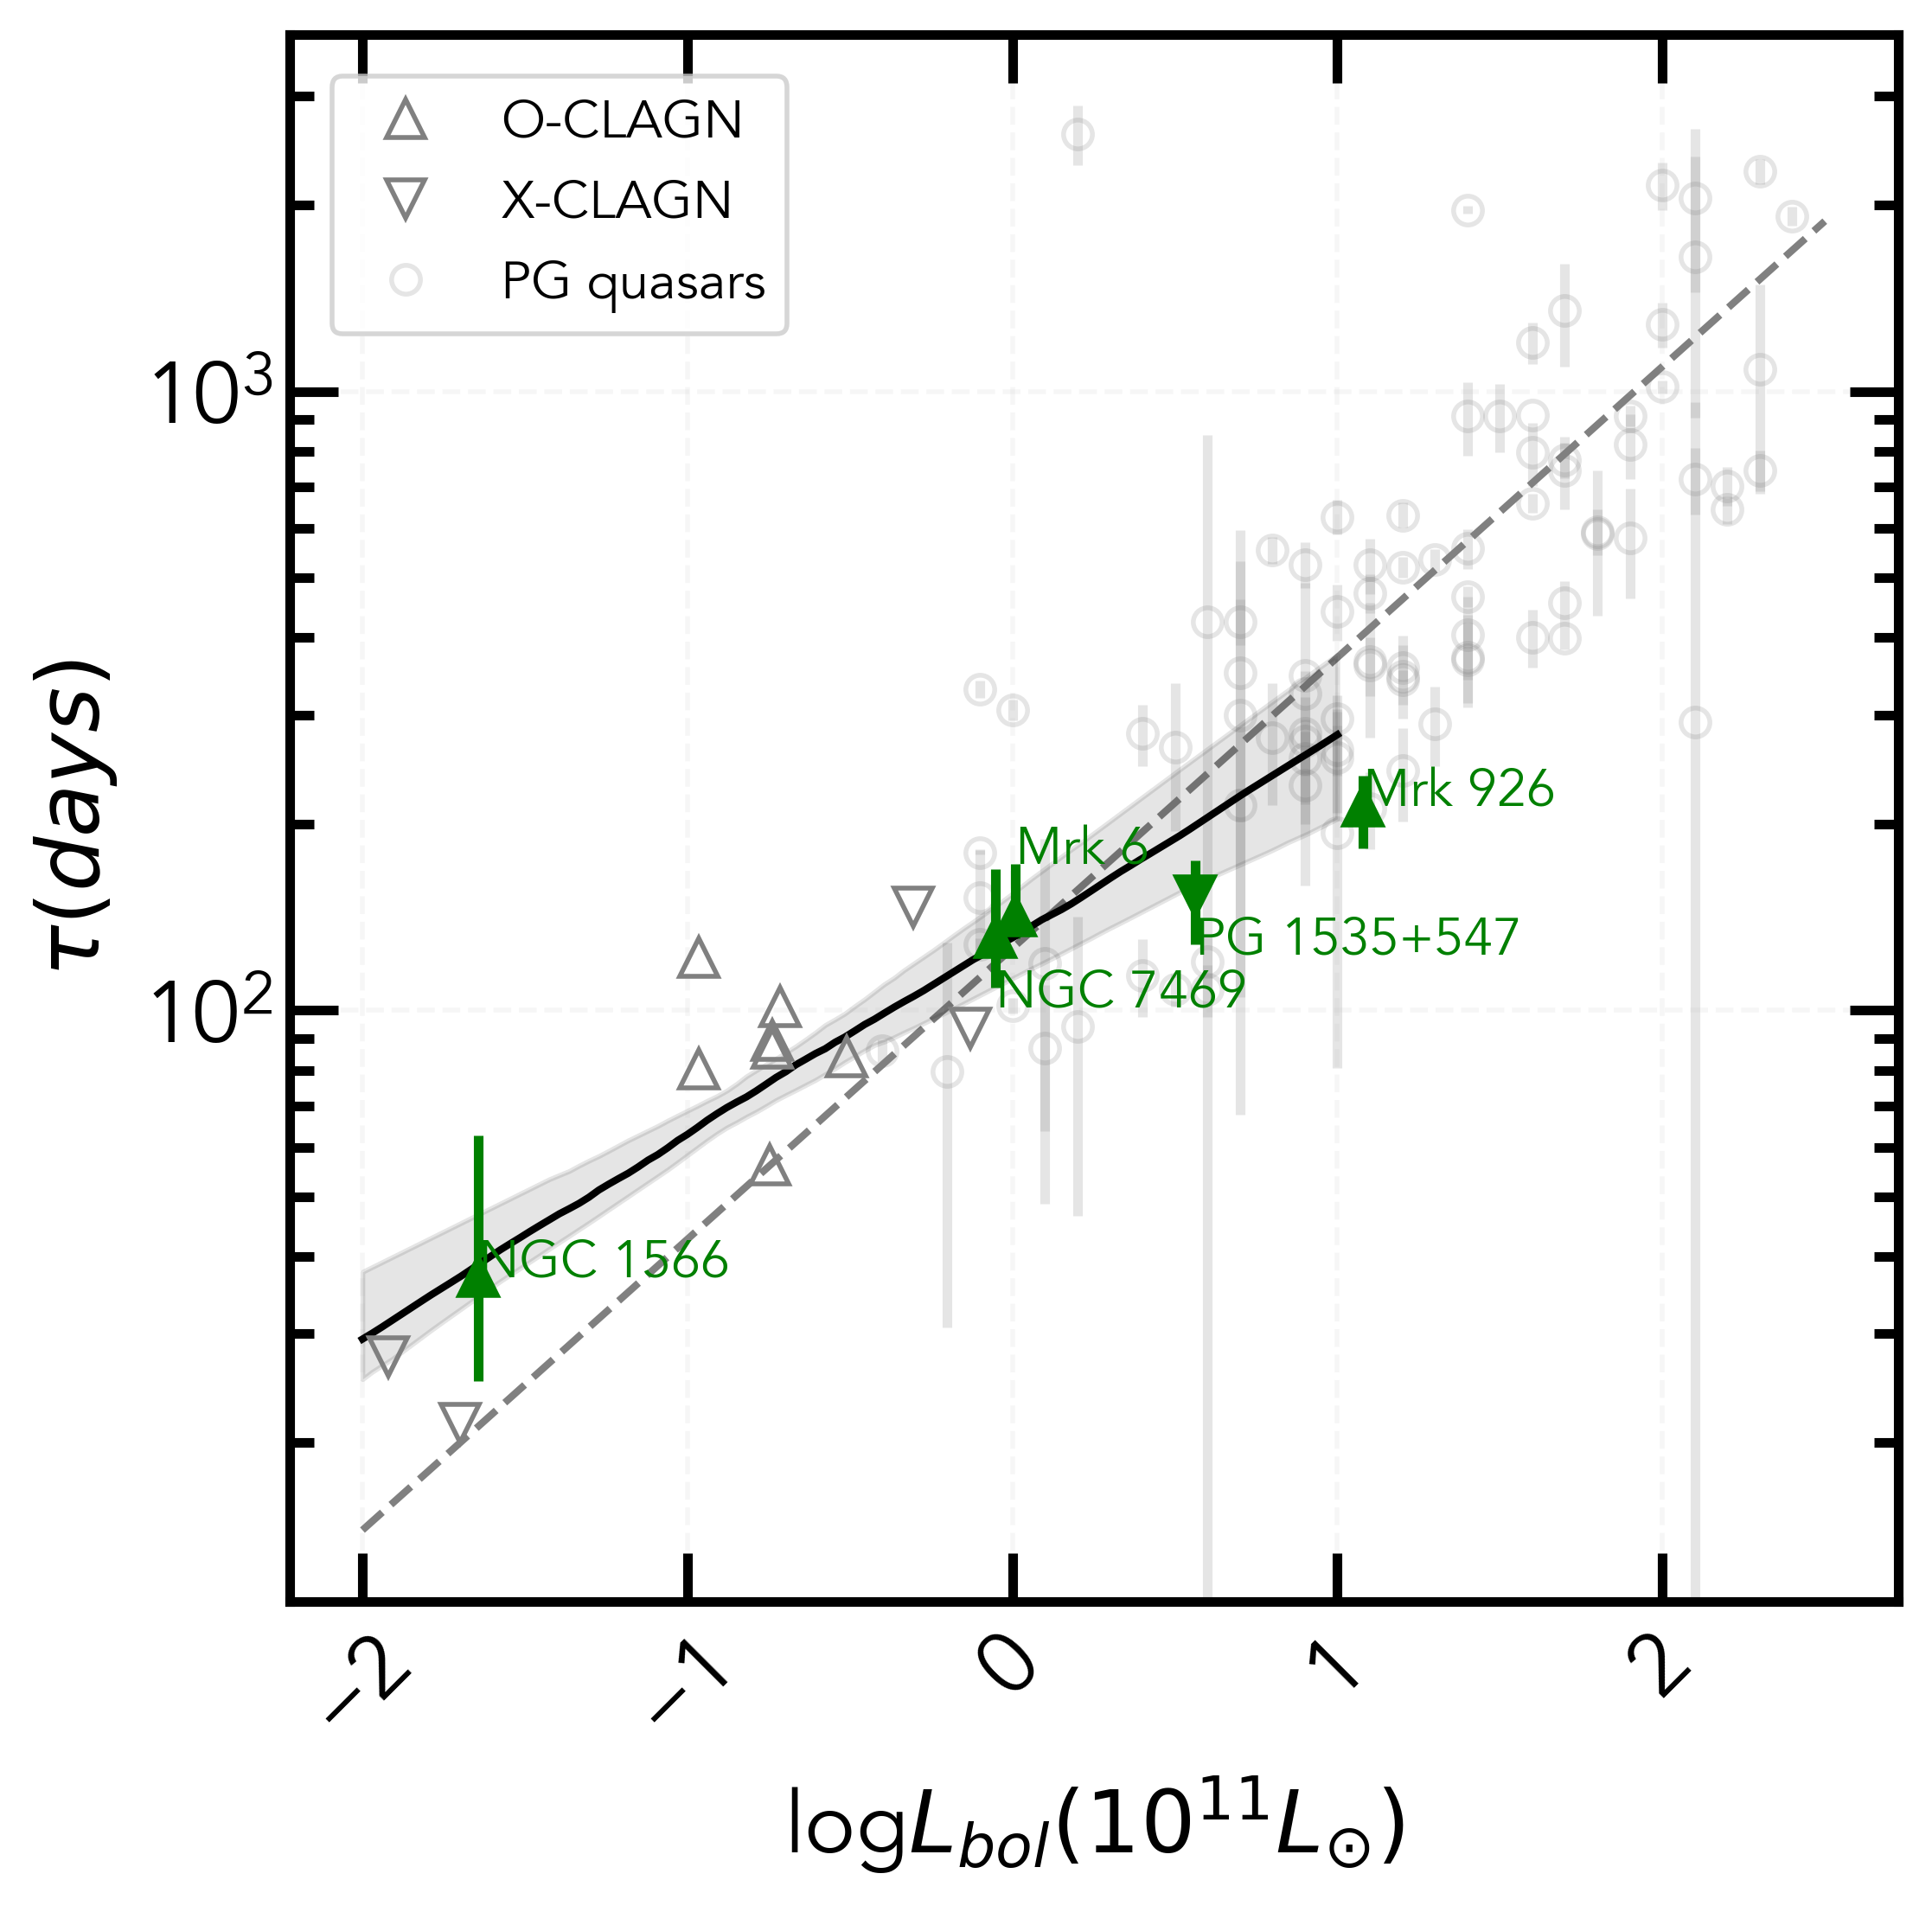
\includegraphics[width=0.45\textwidth]{tau_L_correlation_clagn.png}
    \caption{$\tau$-L correlation for CLAGNs, where $\tau$ is time lag between V band and $W$1 band and L is bolometric luminosity. Grey circles represent PG quasars \citep{2019ApJ...886...33L} for comparison. The dashed line repserent the best fitting of $\tau$-L correlation for PG quasars in \citet{2019ApJ...886...33L}. The straight line is the best fitting for CLAGNs with a scatter in the shadow region.} 
    \label{fig:tau_L}
\end{figure}


\begin{table}
 \caption{Dust reverberation time lag of CLAGNs.
}
 \label{table_lag}
 \begin{center}
 \begin{tabular}{lcccc}
 \hline\hline
Name & log($L_{bol}$) & $\tau$~(days) &Type \\ \hline 
Mrk 590 & 44.13 & $57.9^{+17.8}_{-20.0}$ & O \\
Mrk 6 & 44.59 & $142.1^{+30.0}_{-11.5}$ & O \\
Mrk 926 & 45.66 & $213.8^{+25.3}_{-31.0}$ & O \\
NGC 1566 & 42.94 & $37.1^{+25.7}_{-11.9}$ & O \\
NGC 3516 & 44.19 & $91.1^{+64.0}_{-31.4}$ & O \\
NGC 4051 & 42.61 & $22.3^{+10.4}_{-10.0}$ & X \\
NGC 4151 & 44.08 & $74.4^{+40.8}_{-19.5}$ & O \\
NGC 5548 & 44.66 & $131.2^{+18.6}_{-32.2}$ & O \\
NGC 7469 & 44.53 & $131.2^{+37.9}_{-22.4}$ & X \\
PG 1535+547 & 45.15 & $153.2^{+21.2}_{-25.3}$ & X \\
\hline\hline
\end{tabular}
\end{center}
Note. The table lists source name, bolometric luminosity, dust reverberation time lag between V band and $W$1 band, CLAGN types (``O'' for optical CLAGN and ``X'' for X-ray CLAGN). 
\end{table}


%\begin{figure}
\centering
	% To include a figure from a file named example.*
	% Allowable file formats are eps or ps if compiling using latex
	% or pdf, png, jpg if compiling using pdflatex
	\includegraphics[width=0.5\textwidth]{tau_L_correlation_type.png}
    \caption{$\tau$-L correlation for CLAGNs and quasars, where $\tau$ is time lag between V band and $W$1 band and L is bolometric luminosity. Grey circles represent PG quasars \citep{2019ApJ...886...33L}. The grey dashed line repserent the best fitting of $\tau$-L correlation for PG quasars with a slope of $\sim$ 0.47 in \citet{2019ApJ...886...33L}.
    Stars represent Type 1 AGN \citep[][]{2014ApJ...788..159K,2019ApJ...886...33L}. The time lags for Type 1s are scaled from $\tau_\mathrm{K}$ to $\tau_\mathrm{W1}$ by multiplying a factor of 5/3 according to \citet[][]{2019ApJ...886...33L}. Square represents the type 2 AGN NGC 2110 for X-ray and MIR time lag \citep[see ][]{2020MNRAS.495.2921N}. The black straight line represents the best-fitting for Type 1s, Type 2s, and CLAGNs, with a slope of $\sim$ 0.36. The red dashed lines represent the scatter of $\sim$0.17 dex.  }
    \label{fig:tau_L}. 
\end{figure}


\begin{table}
 \caption{Dust reverberation time lag of CLAGNs.
}
 \label{table_lag}
 \begin{center}
 \begin{tabular}{lccccc}
 \hline\hline
Name & log($L_{bol}/L_{\odot}$) & $\tau$~(days) &Type  & references\\ \hline 
NGC 1566 & 9.91 & $37.1^{+25.7}_{-11.9}$ & O & This work \\
Mrk 6 & 11.01 & $142.1^{+30.0}_{-11.5}$ & O & This work \\
Mrk 926 & 12.08 & $213.8^{+25.3}_{-31.0}$ & O & This work \\
PG 1535+547 & 11.56 & $153.2^{+21.2}_{-25.3}$ & X & This work \\
NGC 2110 & 10.95 & $153.2^{+21.2}_{-25.3}$ & Type 2 & \citet{2020MNRAS.495.2921N} \\
Mrk 335 & 11.03 & $ 167.1 \pm 5.60$ & Type 1 & \citet{2014ApJ...788..159K} \\
Mrk 590 & 10.25 & $ 33.8 \pm 4.20$ & O & \citet{2014ApJ...788..159K} \\
IRAS 03450+0055 & 11.34 & $ 158.3 \pm 5.40$ & Type 1 & \citet{2014ApJ...788..159K} \\
Akn 120 & 11.67 & $ 140.9 \pm 17.20$ & Type 1 & \citet{2014ApJ...788..159K} \\
MCG +08-11-011 & 10.88 & $ 73.5 \pm 1.40$ & Type 1 & \citet{2014ApJ...788..159K} \\
Mrk 79 & 10.77 & $ 65.6 \pm 5.00$ & Type 1 & \citet{2014ApJ...788..159K} \\
Mrk 110 & 11.03 & $ 119.7 \pm 5.50$ & Type 1 & \citet{2014ApJ...788..159K} \\
NGC 3227 & 9.60 & $ 14.6 \pm 0.70$ & Type 1 & \citet{2014ApJ...788..159K} \\
NGC 3516 & 10.03 & $ 73.1 \pm 4.00$ & O & \citet{2014ApJ...788..159K} \\
Mrk 744 & 9.23 & $ 20.0 \pm 2.20$ & Type 1 & \citet{2014ApJ...788..159K} \\
NGC 4051 & 9.08 & $ 16.5 \pm 0.60$ & X & \citet{2014ApJ...788..159K} \\
NGC 4151 & 10.03 & $ 48.3 \pm 0.50$ & O & \citet{2014ApJ...788..159K} \\
NGC 4593 & 9.95 & $ 41.6 \pm 0.90$ & Type 1 & \citet{2014ApJ...788..159K} \\
NGC 5548 & 10.29 & $ 60.9 \pm 0.30$ & O & \citet{2014ApJ...788..159K} \\
Mrk 817 & 11.12 & $ 93.0 \pm 8.90$ & Type 1 & \citet{2014ApJ...788..159K} \\
Mrk 509 & 11.63 & $ 120.7 \pm 1.80$ & Type 1 & \citet{2014ApJ...788..159K} \\
NGC 7469 & 10.69 & $ 88.0 \pm 0.60$ & X & \citet{2014ApJ...788..159K} \\
Mrk 335 & 11.17 & 137.7 & Type 1 & \citet{2019ApJ...886...33L} \\
IRAS 03450+0055 & 11.46 & 129.1 & Type 1 & \citet{2019ApJ...886...33L} \\
MCG +08-11-011 & 11.76 & 89.5 & Type 1 & \citet{2019ApJ...886...33L} \\
Mrk 79 & 10.93 & 74.6 & Type 1 & \citet{2019ApJ...886...33L} \\
Mrk 110 & 11.17 & 63.7 & Type 1 & \citet{2019ApJ...886...33L} \\
NGC 3227 & 9.85 & 7.0 & Type 1 & \citet{2019ApJ...886...33L} \\
NGC 3516 & 10.26 & 53.6 & O & \citet{2019ApJ...886...33L} \\
Mrk 744 & 9.48 & 26.6 & Type 1 & \citet{2019ApJ...886...33L} \\
NGC 4051 & 9.30 & 12.9 & X & \citet{2019ApJ...886...33L} \\
NGC 4151 & 10.26 & 52.2 & O & \citet{2019ApJ...886...33L} \\
NGC 4593 & 10.17 & 62.1 & Type 1 & \citet{2019ApJ...886...33L} \\
NGC 5548 & 10.49 & 50.5 & O & \citet{2019ApJ...886...33L} \\
Mrk 817 & 11.26 & 91.6 & Type 1 & \citet{2019ApJ...886...33L} \\
Mrk 509 & 11.71 & 122.2 & Type 1 & \citet{2019ApJ...886...33L} \\
NGC 7469 & 10.87 & 56.1 & X & \citet{2019ApJ...886...33L} \\
\hline\hline
\end{tabular}
\end{center}
Note. The table lists source name, bolometric luminosity, dust reverberation time lag, CLAGN types (``O'' for optical selected CLAGN and ``X'' for X-ray selected CLAGN) and references. The time lag for type 2 AGN NGC 2110 is between X-ray (2-20 keV) band and $W$1 band. The time lag for NGC 1566 is between V band and $W$1 band in this work. The time lags results from \citet{2014ApJ...788..159K} and \citet{2019ApJ...886...33L} are between V band and K band. 
\end{table}




\section{Conclusion and Discussion} \label{sec:dis}
%\subsection{MIR variability and color}
The majority of CLAGNs shows extreme MIR variability (see \autoref{fig:var_ledd_hist}). The color $W1$-$W2$ distribution of CLAGNs is similar to active quasars, which suggests that AGN rather than the host galaxy mainly contribute to the strong MIR variability.  The distribution of MIR luminosity of CLAGNs is located between the quiescent LLAGN and active QSO. The MIR Eddington scaled luminosity of CLAGNs is centred at $L_{W1}/L_{Edd} \sim $0.5 per cent, which is near to the critical luminosity of type transitions between a radiatively inefficient accretion flow (ADAF) and a thin accretion disk \citep[e.g.][and references therein]{2009MNRAS.399..349G,2014ARA&A..52..529Y}. The correlation between hardness ratio or the photon index ($\Gamma$) from X-ray spectrum and X-ray luminosity \citep[e.g.][]{2020ApJ...890L..29A,2021MNRAS.506.4188L} and X-ray luminosity distribution \citep[e.g.][]{2021MNRAS.508..144G} show significant discrepancy when CLAGNs are type 1 and type 2, which are consistent with the prediction of accretion mode transition. The MIR variability are very likely driven by the intrinsic variation such as accretion rate change. As the intrinsic luminosity drops, the inner disk might transit into ADAF, reducing the supply of ionizing photons to excite the broad line or BLR are not sustainable when the intrinsic accretion rate declines below the critical value, and then AGN would change its optical type from type 1 to type 2. Besides, the disk-wind might influence the X-ray spectrum with the evolution of accretion disk.  When the optical/UV emission from accretion disk changes, the reprocessed IR emission would respond to the variation as the variation signal travels to the torus at the speed of light. The time lag between MIR and optical V band and bolometric lumonisity in both Optical/X-ray CLAGNs follows the $\tau$-L correlation defined in other AGNs (see \autoref{fig:tau_L}), further confirms that the dust echo response to the accretion process. The MIR luminosity distribution and the $\tau$-L correlation also provide the evidence that CLAGNs are in transitional accretion state. 


The ``changing-look'' phenomena were usually accompanied by the outburst (e.g. Mrk 590, NGC 1566, NGC 2617) or rapid dimming (e.g. Mrk 1018) of sources. Those with a significant increase or decline of MIR luminosity are very likely experiencing new ``changing-look'' according to their long-term MIR light curves since the MIR luminosity variation reflect the change of intrinsic accretion rate. For example, the $\Gamma-L$ correlation of Mrk 1018 is still in the negative branch \citep{2021MNRAS.506.4188L}, which is consistent with that in the faint type 1.9 state. However, the increase of MIR luminosity suggests Mrk 1018 might gradually return to type 1 state again in the future. Seyfert 1.5 galaxy Mrk 6 showed rapid decline over one magnitude after the outburst on 2016 in MIR luminosity. Mrk 6 might transit into type 2 since its MIR Eddington scaled luminosity $L_{W1}/L_{Edd} $ reached $\sim 0.16\%$. Mrk 926 showed detectable but weaker broad H$\beta$ component due to high S/N spectra on 9 July 2019 \citep{2021IAUS..356..122W}. The MIR luminosity decline of Mrk 926 suggests the broad H$\beta$ might gradually fully disappear. More spectroscopic observations are needed to confirm the type change and accretion state evolution of those MIR extremely variable CLAGNs.



\begin{acknowledgments}
BL and QW were supported in part by the NSFC (grant U1931203); ZY was supported in part by the Natural Science Foundation of China (grants 11773055 and U1938114), the Youth Innovation Promotion Association of CAS (id 2020265); and WY would like to acknowledge the support in part by the National Program on Key Research and Development Project (grant 2016YFA0400804) and the National Natural Science Foundation of China (grants 11333005 and U1838203).
%\vspace{5mm}
This research has made use of WISE and NEOWISE data products from the NASA/IPAC Infrared Science Archive, which is a joint project of the University of California, Los Angeles, and the Jet Propulsion Laboratory/California Institute of Technology, funded by the National Aeronautics and Space Administration. 

%This research has made use of the NASA/IPAC Extragalactic Database (NED) which is operated by the Jet Propulsion Laboratory, Caltech, under contract with the National Aeronautics and Space Administration.
%This research has made use of MAXI data provided by RIKEN, JAXA and the MAXI team.


\end{acknowledgments}

%% To help institutions obtain information on the effectiveness of their 
%% telescopes the AAS Journals has created a group of keywords for telescope 
%% facilities.
%
%% Following the acknowledgments section, use the following syntax and the
%% \facility{} or \facilities{} macros to list the keywords of facilities used 
%% in the research for the paper.  Each keyword is check against the master 
%% list during copy editing.  Individual instruments can be provided in 
%% parentheses, after the keyword, but they are not verified.



\facilities{\textit{WISE}, Swift (XRT and UVOT), ASAS-SN}%
%, \maxi\, }
%CTIO:1.3m,CTIO:1.5m,CXO}

%% Similar to \facility{}, there is the optional \software command to allow 
%% authors a place to specify which programs were used during the creation of 
%% the manuscript. Authors should list each code and include either a
%% citation or url to the code inside ()s when available.

\software{astropy \citep{2013A&A...558A..33A,2018AJ....156..123A},  
         \sc{javelin}\citep{2011ApJ...735...80Z,2013ApJ...765..106Z}, 
         \sc{pyccf}\citep{1998PASP..110..660P,2018ascl.soft05032S},
          %Cloudy \citep{2013RMxAA..49..137F}, 
          %Source Extractor \citep{1996A&AS..117..393B}
          }

%% Appendix material should be preceded with a single \appendix command.
%% There should be a \section command for each appendix. Mark appendix
%% subsections with the same markup you use in the main body of the paper.

%% Each Appendix (indicated with \section) will be lettered A, B, C, etc.
%% The equation counter will reset when it encounters the \appendix
%% command and will number appendix equations (A1), (A2), etc. The
%% Figure and Table counter will not reset.

\appendix

\section{Appendix information}
%% For this sample we use BibTeX plus aasjournals.bst to generate the
%% the bibliography. The sample631.bib file was populated from ADS. To
%% get the citations to show in the compiled file do the following:
%%
%% pdflatex sample631.tex
%% bibtext sample631
%% pdflatex sample631.tex
%% pdflatex sample631.tex


\bibliographystyle{aasjournal}
\bibliography{ref.bib}
%% This command is needed to show the entire author+affiliation list when
%% the collaboration and author truncation commands are used.  It has to
%% go at the end of the manuscript.
%\allauthors

%% Include this line if you are using the \added, \replaced, \deleted
%% commands to see a summary list of all changes at the end of the article.
%\listofchanges
%\begin{table}
%\newpage
\startlongtable
\begin{deluxetable}{lllllllllllll}
\tablecaption{CLAGN sample with BH mass and \textit{WISE} variability measurements. Sources with at least 20 valid points of \textit{NEOWISE} data are included here. \label{source}}
%\tablewidth{700pt}
\tablewidth{0pt}
\tabletypesize{\scriptsize}
\tablehead{
\colhead{Name} &\colhead{redshift} & \colhead{Type} & \colhead{Ref} & \colhead{log$M_{BH}/M_{\odot}$} & \colhead{Ref} & \colhead{$\sigma_{m W1}$} & \colhead{$<W1>$} & \colhead{$\sigma_{m W2}$} & \colhead{$<W2>$}  & \colhead{$<W1$-$W2>$} & \colhead{$\Delta\,W1$} & \colhead{$\Delta\,W2$} \\
} 
\decimalcolnumbers
\startdata
1H 0419-577 & 0.1040 & X & 1 & 8.6 & 32 & 0.02 & 10.88 & 0.00 & 9.86 & 1.02 & 0.10 & 0.11 \\
2MASS J16171142+0638333 & 0.2291 & O & 2 & 8.0 & 29 & 0.13 & 13.86 & 0.05 & 12.85 & 1.02 & 0.86 & 0.78 \\
2MASS J22053771-0711147 & 0.2950 & O & 2 & 8.0 & 29 & 0.15 & 13.64 & 0.13 & 12.77 & 0.87 & 0.47 & 0.41 \\
2MASX J09381221+0743398 & 0.0220 & O & 3 & 7.5 & 29 & 0.12 & 11.73 & 0.22 & 11.58 & 0.11 & 0.31 & 0.58 \\
2MASX J09483841+4030436 & 0.0468 & O & 3 & 7.5 & 29 & 0.04 & 11.89 & 0.07 & 11.50 & 0.40 & 0.18 & 0.28 \\
3C 390.3 & 0.0561 & O & 4 & 9.3 & 33 & 0.18 & 9.90 & 0.16 & 8.85 & 1.05 & 0.56 & 0.49 \\
ESO 362-G18 & 0.0124 & O & 5 & 7.7 & 34 & 0.09 & 9.88 & 0.09 & 9.27 & 0.60 & 0.29 & 0.33 \\
Fairall 9 & 0.0461 & O & 4 & 8.4 & 35 & 0.06 & 8.99 & 0.03 & 7.99 & 1.00 & 0.25 & 0.16 \\
HE 1136-2304 & 0.0270 & O & 6 & 7.6 & 6 & 0.36 & 10.84 & 0.21 & 10.02 & 0.84 & 0.90 & 0.96 \\
IC 751 & 0.0315 & X & 7 & 8.5 & 7 & 0.03 & 10.76 & 0.00 & 9.95 & 0.82 & 0.06 & 0.10 \\
IRAS 23226-3843 & 0.0359 & O & 8 & 8.2 & 8 & 0.21 & 11.13 & 0.14 & 10.88 & 0.25 & 0.30 & 0.54 \\
Mrk 1018 & 0.0430 & O & 9 & 7.8 & 36 & 0.14 & 10.87 & 0.16 & 10.39 & 0.46 & 0.88 & 1.27 \\
Mrk 530 & 0.0288 & O & 4 & 8.1 & 37 & 0.10 & 8.50 & 0.10 & 7.58 & 0.92 & 0.48 & 0.45 \\
Mrk 590 & 0.0264 & O & 10 & 7.5 & 38 & 0.14 & 10.22 & 0.22 & 9.79 & 0.41 & 0.42 & 0.69 \\
Mrk 6 & 0.0195 & O & 4 & 8.2 & 39 & 0.57 & 8.56 & 0.49 & 7.70 & 0.84 & 1.74 & 1.52 \\
Mrk 609 & 0.0344 & O & 11 & 7.8 & 40 & 0.09 & 10.43 & 0.13 & 9.94 & 0.47 & 0.48 & 0.64 \\
Mrk 926 & 0.0470 & O & 12 & 8.1 & 41 & 0.20 & 9.56 & 0.16 & 8.66 & 0.89 & 0.57 & 0.46 \\
NGC 1097 & 0.0042 & O & 13 & 8.1 & 42 & 0.09 & 8.22 & 0.09 & 8.00 & 0.21 & 0.14 & 0.22 \\
NGC 1365 & 0.0055 & X & 14 & 6.7 & 43 & 0.09 & 7.72 & 0.07 & 7.03 & 0.69 & 0.25 & 0.26 \\
NGC 1566 & 0.0050 & O & 15 & 6.9 & 44 & 0.28 & 8.82 & 0.42 & 8.53 & 0.28 & 1.09 & 1.57 \\
NGC 2617 & 0.0142 & O & 16 & 7.5 & 45 & 0.15 & 10.12 & 0.18 & 9.55 & 0.57 & 0.79 & 1.03 \\
NGC 2992 & 0.0077 & O & 14 & 7.5 & 46 & 0.19 & 8.57 & 0.23 & 7.94 & 0.63 & 0.73 & 1.04 \\
NGC 3065 & 0.0066 & O & 13 & 8.0 & 47 & 0.06 & 9.75 & 0.04 & 9.73 & 0.02 & 0.07 & 0.12 \\
NGC 3516 & 0.0088 & O & 17 & 7.5 & 38 & 0.16 & 8.83 & 0.17 & 8.19 & 0.63 & 0.63 & 0.60 \\
NGC 4051 & 0.0023 & X & 1 & 6.4 & 48 & 0.12 & 8.90 & 0.12 & 8.10 & 0.80 & 0.41 & 0.43 \\
NGC 4151 & 0.0033 & O & 4 & 7.6 & 38 & 0.29 & 7.32 & 0.25 & 6.24 & 1.06 & 1.13 & 0.79 \\
NGC 4388 & 0.0084 & X & 1 & 6.9 & 49 & 0.16 & 9.29 & 0.23 & 8.39 & 0.89 & 0.47 & 0.68 \\
NGC 4395 & 0.0011 & O & 18 & 5.6 & 50 & 0.20 & 12.44 & 0.18 & 11.66 & 0.78 & 0.66 & 0.56 \\
NGC 4507 & 0.0118 & X & 18 & 7.7 & 51 & 0.09 & 8.69 & 0.08 & 7.61 & 1.07 & 0.35 & 0.31 \\
NGC 454 & 0.0122 & X & 1 & 6.2 & 52 & 0.05 & 12.63 & 0.05 & 12.45 & 0.17 & 0.06 & 0.07 \\
NGC 4939 & 0.0104 & X & 19 & 7.5 & 53 & 0.20 & 9.85 & 0.19 & 9.43 & 0.42 & 0.36 & 0.47 \\
NGC 5548 & 0.0172 & O & 20 & 7.5 & 54 & 0.13 & 8.95 & 0.09 & 8.11 & 0.84 & 0.47 & 0.34 \\
NGC 6300 & 0.0037 & X & 21 & 7.0 & 21 & 0.06 & 9.14 & 0.07 & 8.24 & 0.89 & 0.25 & 0.46 \\
NGC 7469 & 0.0163 & X & 20 & 7.3 & 38 & 0.18 & 8.28 & 0.18 & 7.46 & 0.82 & 0.56 & 0.53 \\
NGC 7582 & 0.0053 & O & 4 & 7.7 & 55 & 0.16 & 7.81 & 0.19 & 6.83 & 0.98 & 0.55 & 0.58 \\
NGC 7674 & 0.0290 & X & 22 & 7.6 & 56 & 0.03 & 9.28 & 0.00 & 8.14 & 1.14 & 0.13 & 0.08 \\
PG 1535+547 & 0.0389 & X & 23 & 7.3 & 23 & 0.09 & 9.79 & 0.08 & 8.97 & 0.82 & 0.56 & 0.45 \\
SDSS J030510.60-010431.6       & 0.0450 & O & 24 & 7.3 & 24 & 0.06 & 12.17 & 0.08 & 11.95 & 0.21 & 0.24 & 0.38 \\
SDSS J080020.98+263648.8       & 0.0267 & O & 24 & 7.1 & 24 & 0.21 & 10.09 & 0.24 & 9.33 & 0.75 & 0.80 & 0.88 \\
SDSS J081319.34+460849.5 & 0.0538 & O & 25 & 7.6 & 29 & 0.15 & 12.71 & 0.24 & 12.38 & 0.28 & 0.45 & 0.67 \\
SDSS J081726.41+101210.1 & 0.0458 & O & 26 & 7.5 & 26 & 0.36 & 12.51 & 0.50 & 11.91 & 0.47 & 0.97 & 1.25 \\
SDSS J082323.89+422048.3 & 0.1515 & O & 27 & 8.1 & 27 & 0.08 & 13.59 & 0.09 & 12.90 & 0.69 & 0.57 & 0.82 \\
SDSS J082942.67+415436.9 & 0.1263 & O & 27 & 8.5 & 27 & 0.22 & 11.91 & 0.16 & 11.00 & 0.92 & 0.73 & 0.58 \\
SDSS J090902.35+133019.4 & 0.0499 & O & 25 & 7.3 & 29 & 0.09 & 13.09 & 0.37 & 12.60 & 0.27 & 0.83 & 1.16 \\
SDSS J091531.04+481407.7 & 0.1005 & O & 26 & 7.8 & 57 & 0.13 & 13.25 & 0.15 & 12.73 & 0.50 & 0.65 & 0.86 \\
SDSS J111536.57+054449.7       & 0.0900 & O & 28 & 7.6 & 57 & 0.20 & 13.32 & 0.25 & 12.50 & 0.77 & 1.06 & 1.64 \\
SDSS J113355.93+670107.0 & 0.0397 & O & 26 & 8.2 & 57 & 0.16 & 11.76 & 0.20 & 11.27 & 0.47 & 0.54 & 0.77 \\
SDSS J122550.30+510846.3 & 0.1679 & O & 26 & 8.6 & 57 & 0.08 & 13.01 & 0.12 & 12.29 & 0.72 & 0.65 & 0.73 \\
SDSS J125403.78+491452.8 & 0.0670 & O & 26 & 8.3 & 57 & 0.08 & 12.74 & 0.12 & 12.43 & 0.30 & 0.34 & 0.45 \\
SDSS J131615.95+301552.2       & 0.0492 & O & 24 & 7.1 & 24 & 0.07 & 11.64 & 0.11 & 11.39 & 0.25 & 0.24 & 0.41 \\
SDSS J132457.29+480241.2       & 0.2716 & O & 27 & 8.0 & 29 & 0.09 & 13.64 & 0.01 & 12.87 & 0.77 & 0.30 & 0.23 \\
SDSS J141324.27+530527.0       & 0.4559 & O & 29 & 8.2 & 29 & 0.30 & 13.45 & 0.38 & 12.44 & 0.94 & 1.45 & 1.72 \\
SDSS J153308.02+443208.4 & 0.0367 & O & 26 & 7.6 & 26 & 0.12 & 11.98 & 0.24 & 11.85 & 0.08 & 0.42 & 0.82 \\
SDSS J155440.25+362952.0       & 0.2368 & O & 25 & 8.0 & 25 & 0.07 & 13.73 & 0.01 & 12.91 & 0.82 & 0.84 & 1.24 \\
SDSS J162501.43+241547.3       & 0.0503 & O & 24 & 6.7 & 24 & 0.12 & 12.55 & 0.17 & 12.19 & 0.34 & 0.39 & 0.55 \\
SDSS J163629.66+410222.4       & 0.0474 & O & 24 & 7.0 & 24 & 0.02 & 12.95 & 0.00 & 12.88 & 0.07 & 0.06 & 0.07 \\
SDSS J172322.31+550413.8 & 0.2947 & O & 27 & 8.6 & 27 & 0.11 & 13.45 & 0.16 & 12.58 & 0.83 & 0.30 & 0.28 \\
SDSSJ120447.91+170256.8        & 0.2979 & O & 30 & 8.0 & 30 & 0.21 & 13.88 & 0.14 & 12.70 & 1.21 & 1.03 & 0.70 \\
UGC 3223 & 0.0156 & O & 31 & 8.0 & 31 & 0.08 & 10.82 & 0.14 & 10.59 & 0.21 & 0.25 & 0.46 \\
UGC 4203 & 0.0135 & X & 14 & 6.8 & 43 & 0.03 & 9.96 & 0.02 & 8.60 & 1.36 & 0.14 & 0.09 \\
WISEA J035301.02-062326.2 & 0.0762 & O & 3 & 7.6 & 29 & 0.07 & 13.09 & 0.08 & 12.54 & 0.54 & 0.24 & 0.20 \\
WISEA J084748.28+182440.0 & 0.0848 & O & 3 & 7.7 & 29 & 0.20 & 12.88 & 0.24 & 12.25 & 0.58 & 0.70 & 0.79 \\
WISEA J100323.46+352503.8 & 0.1189 & O & 28 & 8.0 & 57 & 0.30 & 13.27 & 0.29 & 12.44 & 0.81 & 1.14 & 1.33 \\
WISEA J110057.70-005304.4 & 0.3790 & O & 29 & 8.2 & 29 & 0.09 & 13.55 & 0.06 & 12.59 & 0.96 & 0.40 & 0.40 \\
WISEA J113229.14+035729.1 & 0.0909 & O & 28 & 7.9 & 57 & 0.12 & 13.28 & 0.12 & 12.70 & 0.58 & 0.67 & 0.80 \\
WISEA J131930.75+675355.4 & 0.1664 & O & 28 & 7.5 & 57 & 0.08 & 13.61 & 0.07 & 12.85 & 0.76 & 0.25 & 0.33 \\
WISEA J144754.23+283324.1 & 0.1634 & O & 28 & 8.0 & 57 & 0.13 & 12.89 & 0.15 & 12.17 & 0.72 & 0.56 & 0.67 \\
WISEA J154507.52+170950.8 & 0.0483 & O & 29 & 7.4 & 29 & 0.18 & 12.27 & 0.21 & 11.65 & 0.60 & 0.71 & 0.80 \\
WISEA J154529.63+251127.9 & 0.1170 & O & 28 & 8.1 & 57 & 0.14 & 13.18 & 0.17 & 12.56 & 0.60 & 0.52 & 0.58 \\
WISEA J155258.27+273728.5 & 0.0865 & O & 28 & 8.1 & 57 & 0.06 & 13.51 & 0.00 & 12.92 & 0.58 & 0.32 & 0.49 \\
\enddata
%\tablecomments{}
\end{deluxetable}
%\begin{flushleft}
%\hline
Note. The table lists source name, redshift, CLAGN type (``O'' for optical selected CLAGN and ``X'' for X-ray selected CLAGN), mass, references, the variability ($\sigma_m$) of $W1$ and $W2$, the mean magnitude of $W1$ and $W2$, mean color of $W1$-$W2$, maximum magnitude variation ($\Delta\,W1$ and $\Delta\,W2$) of \textit{WISE} data.\\

References. (1)~\citet{2012MNRAS.421.1803M} (2)~\citet{2019ApJ...874....8M} (3)~\citet{2016ApJ...821...33R} (4)~\citet{2019sf2a.conf..509M} (5)~\citet{2018Galax...6...52A} (6)~\citet{2018A&A...619A.168K} (7)~\citet{2016ApJ...820....5R} (8)~\citet{2020A&A...638A..91K} (9)~\citet{2020A&A...644L...5H} (10)~\citet{2020MNRAS.491.4615K} (11)~\citet{2020MNRAS.499.1005W} (12)~\citet{2021IAUS..356..122W} (13)~\citet{2021MNRAS.503.2583S} (14)~\citet{2003MNRAS.342..422M} (15)~\citet{2020MNRAS.498..718O} (16)~\citet{2017OAP....30..117O} (17)~\citet{2021ApJ...909...18F} (18)~\citet{2021MNRAS.507..687J} (19)~\citet{2005MNRAS.356..295G} (20)~\citet{2018ATel11915....1O} (21)~\citet{2020MNRAS.499.5396J} (22)~\citet{2005A&A...442..185B} (23)~\citet{2008A&A...483..137B} (24)~\citet{2020MNRAS.498.3985Y} (25)~\citet{2017ApJ...846L...7S} (26)~\citet{2019ApJ...883...31F} (27)~\citet{2021A&A...650A..33P} (28)~\citet{2018ApJ...862..109Y} (29)~\citet{2020MNRAS.491.4925G} (30)~\citet{2019ApJ...887...15W} (31)~\citet{2020ApJ...901....1W} (32)~\citet{2014A&A...563A..95D} (33)~\citet{2011MNRAS.410.1877S} (34)~\citet{2014MNRAS.443.2862A} (35)~\citet{2017MNRAS.466.1777P} (36)~\citet{2018MNRAS.480.3898N} (37)~\citet{2018MNRAS.478.4214E} (38)~\citet{2013ApJ...773...90G} (39)~\citet{2018MNRAS.481.4542S} (40)~\citet{2010ApJ...720..786L} (41)~\citet{2010A&A...522A..36K} (42)~\citet{2015ApJ...800...63S} (43)~\citet{2017MNRAS.468L..97O} (44)~\citet{2002ApJ...579..530W} (45)~\citet{2019arXiv190904676R} (46)~\citet{2020MNRAS.496.3412M} (47)~\citet{2001ApJ...554..240E} (48)~\citet{2019MNRAS.487..667C} (49)~\citet{2019ApJ...884..106M} (50)~\citet{2005ApJ...632..799P} (51)~\citet{2011AAS...21822816M} (52)~\citet{2009ApJ...690.1322W} (53)~\citet{2017ApJ...850...74K} (54)~\citet{2014MNRAS.445.3073P} (55)~\citet{2018MNRAS.473.5334R} (56)~\citet{2017NatAs...1..727K} (57)~\citet{2021ApJ...907L..21D} 
%\end{flushleft}
%\end{table}








\end{document}

% End of file `sample631.tex'.



